%%%%%
%%%%%  Use LUALATEX, not LATEX.
%%%%%
%%%%
\documentclass[]{VUMIFTemplateClass}

\usepackage{indentfirst}
\usepackage{amsmath, amsthm, amssymb, amsfonts}
\usepackage{mathtools}
\usepackage{physics}
\usepackage{graphicx}
\usepackage{verbatim}
\usepackage[hidelinks]{hyperref}
\usepackage{xcolor,algorithm,algorithmic}
\definecolor{gray}{gray}{0.6}


\usepackage{tcolorbox}

\newcommand{\yellowcomment}[1]{%
    \begin{tcolorbox}[colback=yellow!80, colframe=yellow!80, arc=0pt, outer arc=0pt, boxrule=0pt, left=3pt, right=3pt, top=3pt, bottom=3pt]
        \textbf{\textcolor{red}{COMMENT:}} #1
    \end{tcolorbox}
}

\newcommand{\warningcomment}[1]{%
    \begin{tcolorbox}[colback=yellow!90, colframe=red, arc=0pt, outer arc=0pt, boxrule=2pt, left=5pt, right=5pt, top=5pt, bottom=5pt]
        \Large\textbf{\textcolor{red}{FIX THIS: }} \normalsize #1
    \end{tcolorbox}
}

\newcommand{\goodcomment}[1]{%
    \begin{tcolorbox}[colback=green!20, colframe=green!60, arc=0pt, outer arc=0pt, boxrule=1pt, left=3pt, right=3pt, top=3pt, bottom=3pt]
        \textbf{\textcolor{green!70!black}{GOOD:}} #1
    \end{tcolorbox}
}

\newcommand{\noticecomment}[1]{%
    \begin{tcolorbox}[colback=blue!20, colframe=blue!60, arc=0pt, outer arc=0pt, boxrule=1pt, left=3pt, right=3pt, top=3pt, bottom=3pt]
        \textbf{\textcolor{blue!70!black}{NOTE:}} #1
    \end{tcolorbox}
}

\newcommand{\todocomment}[1]{%
    \begin{tcolorbox}[colback=red!20, colframe=red!60, arc=0pt, outer arc=0pt, boxrule=1pt, left=3pt, right=3pt, top=3pt, bottom=3pt]
        \textbf{\textcolor{orange!70!black}{TODO:}} #1
    \end{tcolorbox}
}

\newcommand{\suggestioncomment}[1]{%
    \definecolor{lime}{RGB}{50,205,50}%
    \begin{tcolorbox}[colback=lime!15, colframe=lime!60, arc=0pt, outer arc=0pt, boxrule=1pt, left=3pt, right=3pt, top=3pt, bottom=3pt]
        \textbf{\textcolor{lime!70!black}{SUGGESTION:}} #1
    \end{tcolorbox}%
}

\usepackage[nottoc]{tocbibind}
\usepackage{tocloft}
\usepackage{longtable}
\usepackage{amssymb}

\usepackage{titlesec}
\newcommand{\sectionbreak}{\clearpage}

\makeatletter
\renewcommand{\fnum@algorithm}{\thealgorithm}
\makeatother
\renewcommand\thealgorithm{\arabic{algorithm} algorithm}

\usepackage{biblatex}
\bibliography{bibliografija}
%% to change the numbering (numeric or alphabetic) of bibliographic sources, make the change in VUMIFTemplateClass.cls, line 139

% Author's MACROS
\newcommand{\EE}{\mathbb{E}\,} % Mean
\newcommand{\ee}{{\mathrm e}}  % nice exponent
\newcommand{\RR}{\mathbb{R}}

\makeatletter
% introduce a 4th-level sectioning command: \subsubsubsection
\newcounter{subsubsubsection}[subsubsection]
\renewcommand\thesubsubsubsection{\thesubsubsection.\arabic{subsubsubsection}}

\providecommand\subsubsubsection{%
    \@startsection{subsubsubsection}{4}{\z@}%
        {-3.25ex\@plus -1ex \@minus -.2ex}%
        {1.5ex \@plus .2ex}%
        {\normalfont\normalsize\bfseries}%
}

% ensure numbering and TOC include this level
\setcounter{secnumdepth}{4}
\setcounter{tocdepth}{4}
\makeatother


\studyprogramme{Software Engineering} %Write your study programme (example – Software engineering, Financial and Actuarial Mathematics, etc.)
\worktype{PS Software Design} % Bachelor's thesis or Master's thesis
\worktitle{PS Sofware Design documentation}
% \secondworktitle{Work Title in Lithuanian}
\workauthor{Tadas Riksas, Darius Spruogis, Gustas Mickus, Julius Jauga}

%There may be more than one author, in which case each author is written from a new line which is added in Titlepage.tex or LongerTitlePage.tex
%\secondauthor{Name Surname} %If present, otherwise delete

\supervisor{Vasilij Savin}
% \reviewer{pedagogical/scientific title Name Surname} %If present, otherwise delete
% \scientificadvisor{pedagogical/scientific title Name Surname} %If present, otherwise delete

\begin{document}
\selectlanguage{english}

\onehalfspacing
\begin{titlepage}
\vskip 20pt
\begin{center}

\includegraphics[scale=0.55]{images/MIF.png}
\end{center}

\makeatletter

\vskip 20pt
\centerline{\bf \large \textbf{VILNIUS UNIVERSITY}}
\vskip 10pt
\centerline{\large \textbf{FACULTY OF MATHEMATICS AND INFORMATICS}}
\vskip 10pt
\centerline{\large \textbf{\MakeUppercase{\@studyprogramme \space study programme}}}

\vskip 80pt
\centerline{\Large \@worktype}
\vskip 20pt
\begin{center}
    {\bf \LARGE \@worktitle}
\end{center}
\begin{center}
    {\bf \Large \@secondworktitle}
\end{center}
\vskip 80pt

\centering{\Large \@workauthor}
\@ifundefined{@secondauthor}{}
{
\vskip 10pt
\centering{\Large \@secondauthor}
}
\vskip 20pt

\centering{
    \begin{tabular}{rcp{.7\textwidth}}
        {\Large Supervisor} & {\Large :} & {\Large \@supervisor}\\[10pt]
        \@ifundefined{@scientificadvisor}{}
            {
                {\Large Scientific advisor} & {\Large :} & {\Large \@scientificadvisor}\\[10pt]
            }
        \@ifundefined{@reviewer}{}
            {
                {\Large Reviewer} & {\Large :} & {\Large \@reviewer}\\[10pt]
            }
    \end{tabular}}


\vskip 110pt

\centerline{\large \textbf{Vilnius}}
\centerline{\large \textbf{\the\year{}}}

\makeatother

\newpage
\end{titlepage}
%\newgeometry{top=2cm,bottom=2cm,right=2cm,left=3cm}
\setcounter{page}{2}


\tableofcontents
\onehalfspacing


\section*{Check list \checkmark}

The suggested structure below is only a recommendation. You can decide to adopt a different flow as long as you cover everything that is relevant for the system under design. One good way of testing it is to designate one person on the team who will take on an implementer's hat and read through the document as if they will have to implement that document.

\begin{enumerate}
    \item Intro
    \item Business flows (with sequence diagrams or flow diagrams)
    \item Package diagrams showing classes/modules of the system - high level architecture
    \item Data model for entity used in the system (recommended class diagrams instead of ER diagrams)
    \item API Contracts for the backend endpoints (with Swagger/Open API)
    \begin{itemize}
        \item HTTP requests with all possible parameters
        \item HTTP responses
        \item HTTP error codes
    \end{itemize}
\end{enumerate}

\subsection*{Submission Requirements}

The team will have to prepare two documents:

\begin{itemize}
    \item \textbf{A shared text document} with all diagrams, descriptions and other relevant technical details needed. This document is shared with the lecturer and the final snapshot past submission deadline will be used for grading. You can use Word, Google Docs or Overleaf to share this document.
    
    \item \textbf{A plaintext document in YAML format} that can be loaded into \href{https://editor.swagger.io/}{https://editor.swagger.io/}. This document is put into your team's repository and the link to your Git repo is provided by the team lead to lecturer.
\end{itemize}

It is expected that your YAML file should load there without syntax errors. If the upload fails, only the visible parts of API Design will be graded.

\subsection*{System-under-design Business Requirements}

We are simulating a Software as a Service startup that you will be running. You are creating software for small and medium businesses in catering (bars/cafe/restaurants) and beauty (barbers/hairdressers/SPA) sectors. Your system needs to support both functionalities; however, feature sets can be regulated by the plan your customers subscribed to.

It is enough to design system that is only operated by business employees where the only input customer provides is payment and contact information for bookings.

This list can be expanded/clarified by additional questions raised by students during the design process. It is not meant to be a complete list from the get-go.

\subsubsection*{Order Functionality}

\begin{itemize}
    \item Employee can create an order
    \item Employee can modify an open order (change items)
    \item Employee cannot modify a closed/paid order
    \item Employee can cancel an open (unpaid/not closed order)
    \item Customer can pay the order by cash, gift card and credit/debit card
    \begin{itemize}
        \item \textbf{BEWARE:} In Lab 2 every team will be asked to implement card payment integration with Stripe payment provider, so you might want to do extra research on how card payment flow works.
    \end{itemize}
    \item Each order should allow split checks (multiple payments).
    \item Customer can add a tip to an order.
    \item Employee can apply a discount to an order.
    \item When order is closed the customer can get the final receipt with all costs, taxes, discounts and service charges calculated and presented
    \begin{itemize}
        \item Different order items can have different taxes applied to them (food vs alcohol as an example)
    \end{itemize}
    \item Paid/closed orders are to be preserved indefinitely.
    \item Closed orders can be refunded and marked as such.
\end{itemize}

\subsubsection*{Services}

\begin{itemize}
    \item Employee can make a reservation for a customer
    \begin{itemize}
        \item Each reservation has time when booked, appointment time, employee, customer, service
    \end{itemize}
    \item Employee can cancel or modify an appointment upon customer request
    \item \textbf{BONUS} - send SMS notification when appointment is created (I recommend AWS SMS functionality for that)
\end{itemize}

\subsubsection*{System Management Functionality}

\begin{itemize}
    \item \textbf{BONUS:} Inventory management (should be integrated with order management and have quantities reduced when bought)
    \item Tax Management (create/edit/delete)
    \begin{itemize}
        \item Change of the tax entry (like VAT) should not affect any historical records
    \end{itemize}
    \item Service charge/Tip/Gratuity Management
    \begin{itemize}
        \item Change of the service charge item should not affect any historical records
    \end{itemize}
    \item Product/Menu Item Management (create/edit/delete)
    \item Each product can have variations (e.g. coffee with milk, decaf, vegan milk)
    \item Each Service has an employee associated with it
    \item Discount Management
    \begin{itemize}
        \item Discounts can be applied to a specific product or the whole order
        \item Discounts can be time-limited
    \end{itemize}
    \item User Management (can create/delete/edit users)
    \begin{itemize}
        \item Only business owner can edit employees/users of their business
        \item SuperAdmin (IT Support) can edit anyone
        \item All actions should be performed only by logged-in and authorized users
    \end{itemize}
    \item Merchant/Business management
    \begin{itemize}
        \item Each merchant/business has an owner user, address, contact info (phone, email), name and other relevant details
    \end{itemize}
\end{itemize}


%% Acknowledgements Section
\sectionnonumnocontent{Acknowledgements}
The authors are thankful to the lecturer Vasilij Savin for his guidance and
support throughout the project.


% Lets first give some context to copilot
% #  **Business Management System - Project Summary**

% ##  **Project Overview**
% Building a **multi-tenant SaaS platform** for small service businesses (bars, restaurants, spas, salons) to manage their operations, appointments, orders, and payments in one unified system.

% ##  **Core Business Domains**

% ### ️ **Order Management** (Bars/Restaurants)
% - **Table-based ordering** with real-time modifications
% - **Split bills**, tips, discounts, and multiple payment methods
% - **Menu management** with item variations (e.g., coffee types, milk options)
% - **Inventory tracking** and stock management

% ###  **Services Management** (Spas/Salons)  
% - **Appointment scheduling** with time slot booking
% - **Employee availability** and conflict prevention
% - **Service catalog** (massages, haircuts, treatments)
% - **SMS notifications** for confirmations and reminders

% ## ️ **Technical Requirements**

% ### **Multi-tenancy Architecture**
% - Single database supporting **multiple businesses**
% - Data isolation between different business tenants
% - Super admin access for system management

% ### **Data Model Criticalities**
% - **Historical data preservation** (price/tax changes must NOT affect past records)
% - **Soft deletion** instead of physical data removal
% - **Calculated fields** handled in application layer, not database

% ### **Key Integration Points**
% - **Payment processing** (Stripe integration)
% - **SMS gateway** for appointment notifications
% - **Role-based authentication** (Customer, Employee, Manager, Admin)

% ##  **Current Focus: Business Flow Division**
% We're analyzing and documenting business workflows across **4 functional domains**:
% 1. **Core Service Delivery & Booking**
% 2. **Customer & Business Management** 
% 3. **Communication & Operations**
% 4. **Payments & Analytics**

% ##  **Academic Context**
% This is for a **software design course** where we're creating technical specifications before implementation. The project emphasizes **proper documentation, data modeling, and API design** following software engineering best practices.

% ##  **Current Task**
% Dividing business flow documentation among team members while maintaining **consistency, clear boundaries, and minimal dependencies** between work streams.

% ---
% **Key Constraint:** The system must handle **both order-based (restaurants) and appointment-based (spas) businesses** with overlapping but distinct workflows.


\section*{Introduction}
This document outlines the software design for a multtenant SaaS platform
aimed at small to medium business that consentrate on order delivery such as
bars, restaurants and services such as spas and salons. The platform will
provide a unified system for managing operations, appointments, orders, and
payments.


% ========================================================================
% FUNCTIONAL DOMAIN SEPARATION
% ========================================================================

% ------------------------------------------------------------------------
% DOMAIN INTERACTIONS
% ------------------------------------------------------------------------

% RESTAURANT ↔ MANAGEMENT
% - Employee assignments to tables/shifts
% - Financial data aggregation
% - Customer profile updates

% SERVICES ↔ MANAGEMENT
% - Employee scheduling and availability
% - Appointment revenue tracking
% - Customer service history

% RESTAURANT ↔ SERVICES (for hybrid businesses)
% - Shared customer profiles
% - Combined service packages
% - Unified payment processing

% NOTE: This separation allows each domain to be developed independently
% while maintaining clear integration points for businesses that operate
% across multiple domains.

\section{Business Flows}

We will first start with business flows by describing the business process we are automating. We will
seperate the business flows into 3 main domains for clarity:
\begin{itemize}
    \item Order Management (Bars/Restaurants)
    \item Services Management (Spas/Salons)
    \item Business Management
\end{itemize}
These domains will communicate in this simple way:
\begin{itemize}
    \item Order Management <-> Business Management
    \item Services Management <-> Business Management
\end{itemize}

We will try to write the business flows and then identify the entities,
components and actions needed to implement these business flows.

% example of how to analyze a business flow
% Autoshop business flow

%     • Client arrives at the autoshop
%     • Mechanic engages new client and asks about the reason for the visit
%     • Client fills in the intake form (contact info, car plates, VIN, complaints/issues, etc)
%     • Mechanic gives initial estimate for time and cost of the fix
%     • Client accepts the quote and gives car keys to the mechanic
%     • Mechanic moves car to the parking lot for cars awaiting repairs
%     • Mechanic initiates repairs (possible uncovering additional issues)
%     • Mechanic orders required spare parts OR Mechanics retrieves needed parts from storage
%     • Mechanic contacts client and provides new estimate for cost and time of repairs
%     • Client approves the update quote
%     • Mechanic completes the repairs
%     • Mechanic moves car to the parking lot of cars awaiting pick up.
%     • Client arrives, pays for the repairs and departs
%     • Mechanic adds closing notes to the fix order and closes the order

% Tables/Entities
% Car
% Employee
% Service? Repair Type performed
% Repairs by order
% Spare parts
% Autoshop
% Inventory

% Components
% Order Management (Order, Payments)
% Employee Management
% Inventory (Spare parts, Inventory)
% Catalogue/Offering (Service? Repair Type performed, Repairs by order)


% Actions
% Client fills in the intake form
% Client accepts the quote
% Client approves the update quote
% Client pays for the repairs


\subsection{Order Management (Bars/Restaurants)}

\noticecomment{In a real system, you might need to consider how orders are communicated (e.g., a screen in the kitchen, notifications), but this is left as a design decision for the team.}

% ------------------------------------------------------------------------------
% ORDER DOMAIN
% (Related to bars, restaurants, cafes — places where customers place orders for items like food and drinks)
%
% Use Case          | Description
% ------------------|--------------------------------------------------------------------
% Create Order      | Employee creates a new order for a customer (e.g., at a table).
% Modify Order      | Add, remove, or update items in an open order.
% Close Order       | Finalize the order when the customer is done.
% Pay Order         | Process payment (cash, card, gift card, split payment).
% Apply Discount    | Specify discounts can be applied to specific products OR entire orders
% Add Tip           | Allow the customer to add a tip to the bill.
% Cancel Order      | Cancel an open order before payment.
% Refund Order      | Process a refund for a paid order (e.g., due to complaint).
% Print Receipt     | Generate a final receipt with items, taxes, discounts, and totals.
% Split Check       | Split the bill among multiple customers.
% Handle Different Tax Rates per Item | Apply different tax rates (e.g., food vs. alcohol).
% Refund Order      | Process refund for closed/paid orders and mark them as refunded.
% Preserve Historical Orders | Keep closed/paid orders indefinitely without modification
% ------------------------------------------------------------------------------


\begin{longtable}{p{0.25\linewidth} p{0.70\linewidth}}
\caption{Use cases for the Order Management domain} \\
\textbf{Use case} & \textbf{Description} \\
\hline
\endfirsthead

\multicolumn{2}{c}{{\tablename\ \thetable{} -- Continued from previous page}} \\
\textbf{Use case} & \textbf{Description} \\
\hline
\endhead

\multicolumn{2}{c}{{Continued on next page}} \\
\endfoot

\endlastfoot

Client Seating (Available) &
\begin{minipage}[t]{\linewidth}
Employee checks seating via POS \& backend. If available, employee assigns a table and confirms with client.
\end{minipage} \\[6pt]
\multicolumn{2}{@{}c@{}}{\color{gray}\rule{0.95\linewidth}{0.4pt}} \\[6pt]

Client Seating (Not Available) &
\begin{minipage}[t]{\linewidth}
Employee checks seating via POS \& backend, finds no seats available, and informs client.
\end{minipage} \\[6pt]
\multicolumn{2}{@{}c@{}}{\color{gray}\rule{0.95\linewidth}{0.4pt}} \\[6pt]

Place Order &
\begin{minipage}[t]{\linewidth}
Client requests menu, places an order via employee. POS \& backend validate items, stock, and combinations. If valid, client confirms; else corrections are requested.
\end{minipage} \\[6pt]
\multicolumn{2}{@{}c@{}}{\color{gray}\rule{0.95\linewidth}{0.4pt}} \\[6pt]

Modify Order &
\begin{minipage}[t]{\linewidth}
Client requests to update an existing order. Employee updates through POS, backend validates. On success, order is updated; on failure, errors are shown for correction.
\end{minipage} \\[6pt]
\multicolumn{2}{@{}c@{}}{\color{gray}\rule{0.95\linewidth}{0.4pt}} \\[6pt]

Cancel Order &
\begin{minipage}[t]{\linewidth}
Client requests to cancel an existing not completed order. Employee cancels through POS, backend validates that it is not completed. On success, order is updated; on failure, errors are shown.
\end{minipage} \\[6pt]
\multicolumn{2}{@{}c@{}}{\color{gray}\rule{0.95\linewidth}{0.4pt}} \\[6pt]

Mark items as delivered for table &
\begin{minipage}[t]{\linewidth}
The employee selects a table. The order with items are retrieved for that table, which is then displayed in the POS. The employee selects items to mark as delivered. The item status is updated in the backend server, and a confirmation is displayed in the POS.
\end{minipage} \\[6pt]
\multicolumn{2}{@{}c@{}}{\color{gray}\rule{0.95\linewidth}{0.4pt}} \\[6pt]

\end{longtable}

\subsubsection{Order client seating(available)}

Flow:
\begin{itemize}
\setlength{\itemsep}{2pt}
\setlength{\parskip}{0pt}
\setlength{\parsep}{0pt}
\item Client enters the restaurant/bar.
\item Employee greets the Client.
\item Employee requests available seating options from the POS system.
\item POS system queries the Backend Server for seating availability.
\item Backend Server returns available seating options to the POS.
\item POS displays seating options to the Employee.
\item Employee suggests available seating options to the Client.
\item Client chooses a seating option.
\item Employee assigns the Client to a table using the POS system.
\item POS system sends the table assignment to the Backend Server for saving and validation.
\item If validation succeeds:
\begin{itemize}
\item Backend Server confirms the assignment to the POS.
\item POS confirms table assignment to the Employee.
\item Employee guides the Client to the assigned table.
\end{itemize}
\item If validation fails:
\begin{itemize}
\item Backend Server returns a failure message to the POS.
\item POS notifies the Employee that assignment failed.
\item Employee informs the Client that the table is unavailable and suggests alternatives or waiting.
\end{itemize}
\end{itemize}

Tables/Entities:
\begin{itemize}
\setlength{\itemsep}{2pt}
\setlength{\parskip}{0pt}
\setlength{\parsep}{0pt}
\item Client
\item Table
\end{itemize}

Components:
\begin{itemize}
\setlength{\itemsep}{2pt}
\setlength{\parskip}{0pt}
\setlength{\parsep}{0pt}
\item Seating Management
\end{itemize}

Actions:
\begin{itemize}
\setlength{\itemsep}{2pt}
\setlength{\parskip}{0pt}
\setlength{\parsep}{0pt}
\item Greet client
\item Request available seating options
\item Retrieve and display seating availability
\item Assign client to table
\item Validate table assignment (availability and conflicts)
\item Confirm table assignment
\item Notify failure and suggest alternatives
\end{itemize}

\begin{figure}[H]
    \centering
    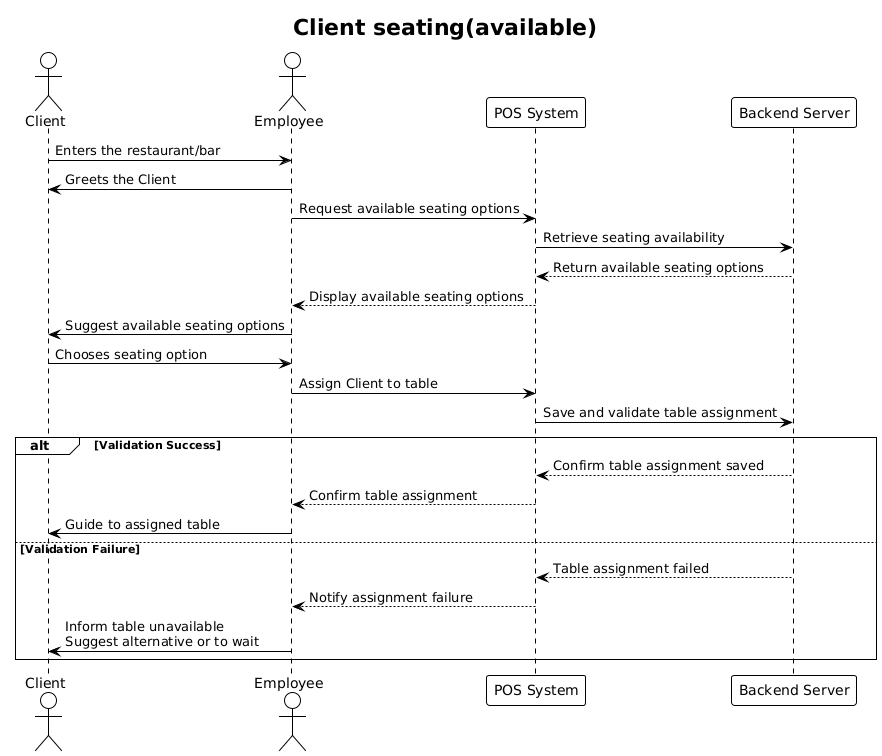
\includegraphics[width=0.8\textwidth]{images/diagrams/orders/order_client_seating_available.png}
    \caption{Client Seating(available) Sequence Diagram}
    \label{fig:client_seating_available_sequence}
\end{figure}

\subsubsection{Order client seating (not available) business flow}

Flow:
\begin{itemize}
\setlength{\itemsep}{2pt}
\setlength{\parskip}{0pt}
\setlength{\parsep}{0pt}
\item Client enters the restaurant/bar.
\item Employee greets the Client.
\item Employee requests available seating options from the POS system.
\item POS system queries the Backend Server for seating availability.
\item Backend Server returns availability data indicating no tables are free.
\item POS displays “no available seating” to the Employee.
\item Employee informs the Client that no seating is currently available.
\end{itemize}

Tables/Entities:
\begin{itemize}
\setlength{\itemsep}{2pt}
\setlength{\parskip}{0pt}
\setlength{\parsep}{0pt}
\item Client
\item Table
\end{itemize}

Components:
\begin{itemize}
\setlength{\itemsep}{2pt}
\setlength{\parskip}{0pt}
\setlength{\parsep}{0pt}
\item POS System (Employee-facing system to check seating availability)
\item Backend Server (handles seating availability queries)
\item Seating Management (Tables + availability status)
\item Employee Interface (to communicate availability to Client)
\end{itemize}

Actions:
\begin{itemize}
\setlength{\itemsep}{2pt}
\setlength{\parskip}{0pt}
\setlength{\parsep}{0pt}
\item Greet client
\item Request seating availability
\item Retrieve seating data
\item Display “no available seating”
\item Inform client that no seating is available
\end{itemize}

\begin{figure}[H]
    \centering
    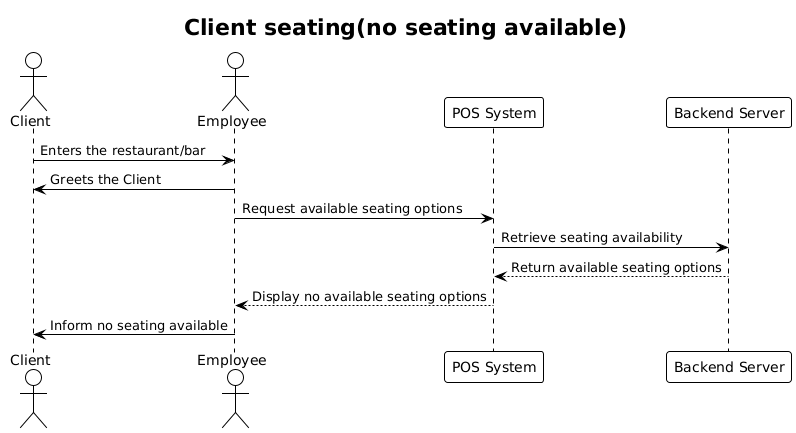
\includegraphics[width=0.8\textwidth]{images/diagrams/orders/order_client_seating_not_available_sequence.png}
    \caption{Client Seating(not available) Sequence Diagram}
    \label{fig:client_seating_not_available_sequence}
\end{figure}

\subsubsection{Place Order Business Flow}

Flow:
\begin{itemize}
\setlength{\itemsep}{2pt}
\setlength{\parskip}{0pt}
\setlength{\parsep}{0pt}
\item Client asks the Employee for the menu.
\item Employee provides the menu to the Client (physical or digital).
\item Client makes an order request to the Employee.
\item Employee inputs the order into the POS system.
\item POS sends the order request to the Backend Server for validation and creation.
\item Backend Server validates the request:
\begin{itemize}
\item Checks stock availability.
\item Validates attribute or variation combinations (e.g., sizes, add-ons).
\end{itemize}
\item If validation succeeds:
\begin{itemize}
\item Backend Server creates a pending order linked to the Client’s table.
\item Backend Server confirms the order to the POS.
\item POS displays the order confirmation to the Employee.
\item Employee informs the Client that the order has been confirmed.
\end{itemize}
\item If validation fails:
\begin{itemize}
\item Backend Server sends validation errors to the POS.
\item POS displays the errors to the Employee.
\item Employee informs the Client and requests corrections or adjustments.
\end{itemize}
\end{itemize}

Tables/Entities:
\begin{itemize}
\setlength{\itemsep}{2pt}
\setlength{\parskip}{0pt}
\setlength{\parsep}{0pt}
\item Client
\item Employee
\item Menu
\item Order
\item Order Item 
\item Inventory
\end{itemize}

Components:
\begin{itemize}
\setlength{\itemsep}{2pt}
\setlength{\parskip}{0pt}
\setlength{\parsep}{0pt}
\item Menu Management (Menu + Item availability)
\item Order Management (Orders + Order Items)
\end{itemize}

Actions:
\begin{itemize}
\setlength{\itemsep}{2pt}
\setlength{\parskip}{0pt}
\setlength{\parsep}{0pt}
\item Provide menu
\item Input order
\item Validate stock availability
\item Validate item variations/attributes
\item Create pending order tied to Client’s table
\item Confirm order success
\item Return errors if validation fails
\item Inform Client of result
\end{itemize}

\begin{figure}[H]
    \centering
    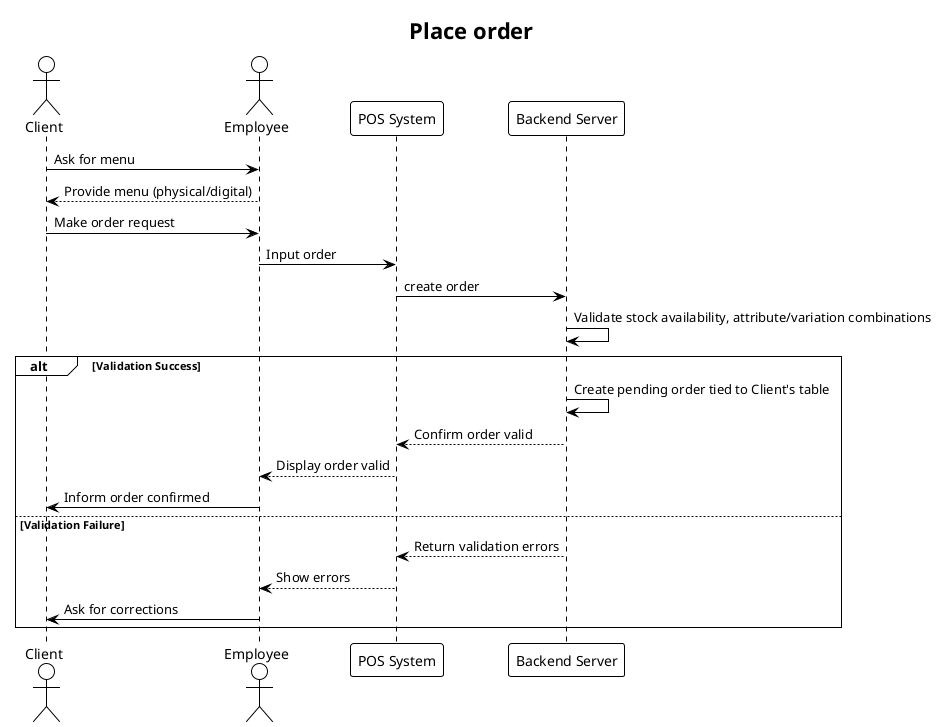
\includegraphics[width=0.8\textwidth]{images/diagrams/orders/order_place_order_sequence.png}
    \caption{Place Order Sequence Diagram}
    \label{fig:place_order_sequence}
\end{figure}

\subsubsection{Update Order Business Flow}

Flow:
\begin{itemize}
\setlength{\itemsep}{2pt}
\setlength{\parskip}{0pt}
\setlength{\parsep}{0pt}
\item Client requests an update to an existing order from the Employee.
\item Employee initiates the update in the POS system.
\item POS system sends the update request to the Backend Server for validation and processing.
\item If the update is successful:
\begin{itemize}
\item Backend Server confirms the update to the POS.
\item POS displays the updated order details to the Employee.
\item Employee informs the Client that the update has been completed.
\end{itemize}
\item If the update fails:
\begin{itemize}
\item Backend Server returns validation errors to the POS.
\item POS displays the errors to the Employee.
\item Employee informs the Client and asks for corrections or adjustments.
\end{itemize}
\end{itemize}

Tables/Entities:
\begin{itemize}
\setlength{\itemsep}{2pt}
\setlength{\parskip}{0pt}
\setlength{\parsep}{0pt}
\item Client
\item Employee
\item Order 
\item Order Item 
\end{itemize}

Components:
\begin{itemize}
\setlength{\itemsep}{2pt}
\setlength{\parskip}{0pt}
\setlength{\parsep}{0pt}
\item Order Management (Orders + Order Items)
\end{itemize}

Actions:
\begin{itemize}
\setlength{\itemsep}{2pt}
\setlength{\parskip}{0pt}
\setlength{\parsep}{0pt}
\item Request order update
\item Validate update request
\item Apply changes to order
\item Confirm update success
\item Return validation errors if update fails
\item Inform Client of results
\end{itemize}

\begin{figure}[H]
    \centering
    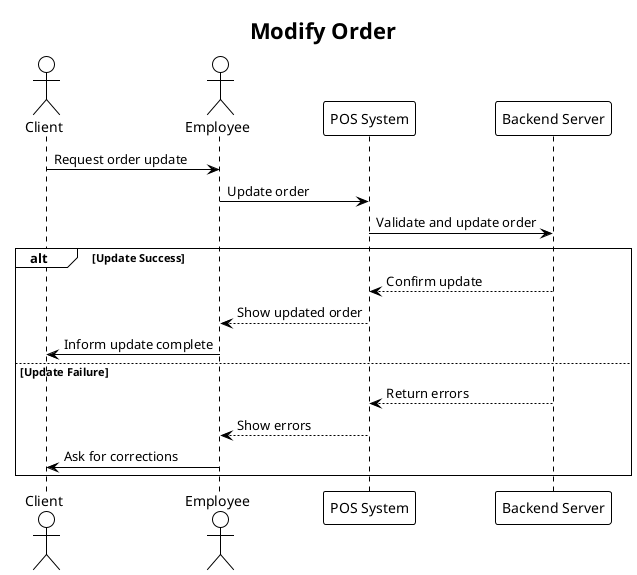
\includegraphics[width=0.8\textwidth]{images/diagrams/orders/order_modify_order_sequence.png}
    \caption{Modify Order Sequence Diagram}
    \label{fig:modify_order_sequence}
\end{figure}

\subsubsection{Order cancellation}

Flow:
\begin{itemize}
\setlength{\itemsep}{2pt}
\setlength{\parskip}{0pt}
\setlength{\parsep}{0pt}
\item Client requests an order cancellation from the Employee.
\item Employee initiates cancellation in the POS system.
\item POS system forwards the cancellation request to the Backend Server.
\item If the order is not yet completed/paid:
\begin{itemize}
\item Backend Server confirms cancellation to the POS.
\item POS shows successful cancellation to the Employee.
\item Employee informs the Client that the order has been canceled.
\end{itemize}
\item If the order has already been completed/paid:
\begin{itemize}
\item Backend Server refuses the cancellation.
\item POS shows the refusal message to the Employee.
\item Employee informs the Client that the cancellation is not allowed.
\end{itemize}
\end{itemize}

Tables/Entities:
\begin{itemize}
\setlength{\itemsep}{2pt}
\setlength{\parskip}{0pt}
\setlength{\parsep}{0pt}
\item Client
\item Employee
\item Order 
\end{itemize}

Components:
\begin{itemize}
\setlength{\itemsep}{2pt}
\setlength{\parskip}{0pt}
\setlength{\parsep}{0pt}
\item Order Management
\end{itemize}

Actions: 
\begin{itemize}
\setlength{\itemsep}{2pt}
\setlength{\parskip}{0pt}
\setlength{\parsep}{0pt}
\item Request cancellation
\item Validate order status (completed/paid or not)
\item Cancel order (if eligible)
\item Refuse cancellation (if already completed/paid)
\item Inform Employee
\end{itemize}

\begin{figure}[H]
    \centering
    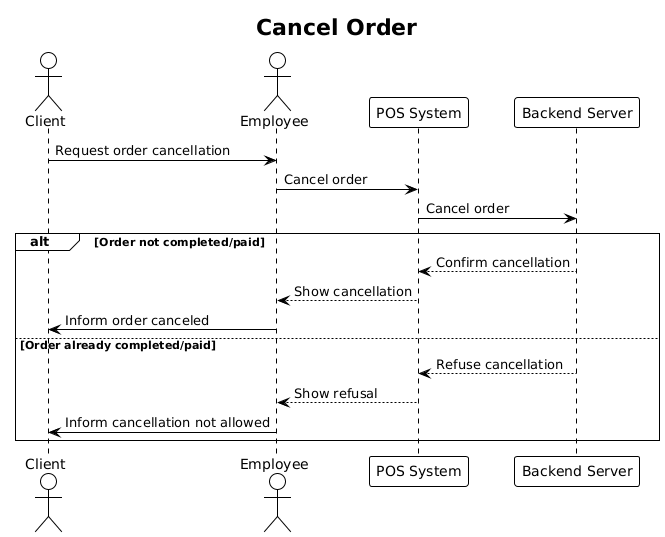
\includegraphics[width=0.8\textwidth]{images/diagrams/orders/order_cancel_order_sequence.png}
    \caption{Cancel Order Sequence Diagram}
    \label{fig:cancel_order_sequence}
\end{figure}

\subsubsection{Mark Items as Delivered for Table Business Flow}

Flow:
\begin{itemize}
\setlength{\itemsep}{2pt}
\setlength{\parskip}{0pt}
\setlength{\parsep}{0pt}
\item Employee selects a table in the POS system.
\item POS system requests open orders for the selected table from the Backend Server.
\item Backend Server returns a list of items associated with that table’s open orders.
\item Employee selects specific items and marks them as delivered in the POS system.
\item POS system sends an update request to the Backend Server, setting the status of the selected items to \texttt{delivered}.
\item Backend Server confirms that the items’ statuses have been updated.
\item POS system displays a delivery confirmation to the Employee.
\end{itemize}

Tables/Entities:
\begin{itemize}
\setlength{\itemsep}{2pt}
\setlength{\parskip}{0pt}
\setlength{\parsep}{0pt}
\item Employee
\item Table 
\item Order
\item Order Item
\end{itemize}

Components:
\begin{itemize}
\setlength{\itemsep}{2pt}
\setlength{\parskip}{0pt}
\setlength{\parsep}{0pt}
\item Order Management
\end{itemize}

Actions:
\begin{itemize}
\setlength{\itemsep}{2pt}
\setlength{\parskip}{0pt}
\setlength{\parsep}{0pt}
\item Select table
\item Retrieve open orders for table
\item Display items to Employee
\item Mark items as delivered
\item Update item status in Backend Server
\item Confirm update to Employee
\end{itemize}

\begin{figure}[H]
    \centering
    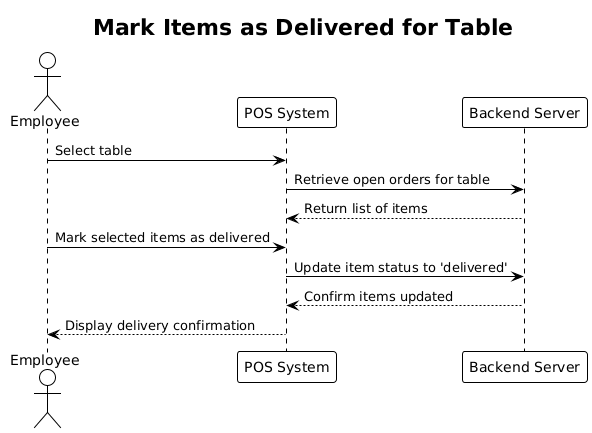
\includegraphics[width=0.8\textwidth]{images/diagrams/orders/order_mark_items_delivered_sequence.png}
    \caption{Mark Items as Delivered Sequence Diagram}
    \label{fig:mark_items_delivered_sequence}
\end{figure}


\subsection{Services Management (Spas/Salons)}

% ------------------------------------------------------------------------------
% Service Domain
% (Related to appointment-based businesses like spas, barbers, massage centers)
%
% Use Case             | Description
% ---------------------|-----------------------------------------------------------------
% Create Appointment   | Employee schedules a service for a customer (date, time, employee).
% Modify Appointment   | Change time, employee, service, date, or assigned employee.
% Cancel Appointment   | Cancel a scheduled service.
% Check Availability   | Verify if an employee is free at a given time.
% Send SMS Reminder    | Automatically send an SMS to the customer before the appointment.
% Assign Employee      | Assign a specialist to a service.
% Mark Service as Done | Record that the service has been completed.
% ------------------------------------------------------------------------------

\noticecomment{The employee that registers the customer doesnt necessarily need to service the customer themselves (think of spas). However smaller businesses (like haircut saloons) employees may both register and service the customer themselves.}

We have identified the following use cases for the services management domain:

\vspace{1cm}
\begin{longtable}{p{0.25\linewidth} p{0.70\linewidth}}
\caption{Use cases for the Services Management domain} \\
\textbf{Use case} & \textbf{Description} \\
\hline
\endfirsthead

\multicolumn{2}{c}{{\tablename\ \thetable{} -- Continued from previous page}} \\
\textbf{Use case} & \textbf{Description} \\
\hline
\endhead

\multicolumn{2}{c}{{Continued on next page}} \\
\endfoot

\endlastfoot

Create appointment &
\begin{minipage}[t]{\linewidth}
Employee or customer schedules a service for a customer by selecting service, date/time and (optionally) employee; system reserves the slot, records booking metadata and sends confirmation.
\end{minipage} \\[6pt]
\multicolumn{2}{@{}c@{}}{\color{gray}\rule{0.95\linewidth}{0.4pt}} \\[6pt]

Modify appointment &
\begin{minipage}[t]{\linewidth}
Change appointment details (time, service, date, assigned employee); system validates availability, preserves historical record of changes and notifies affected parties.
\end{minipage} \\[6pt]
\multicolumn{2}{@{}c@{}}{\color{gray}\rule{0.95\linewidth}{0.4pt}} \\[6pt]

Cancel appointment &
\begin{minipage}[t]{\linewidth}
Customer or staff cancels an appointment; system frees the slot, applies cancellation rules (refund/deposit handling if applicable) and sends notifications.
\end{minipage} \\[6pt]
\multicolumn{2}{@{}c@{}}{\color{gray}\rule{0.95\linewidth}{0.4pt}} \\[6pt]

Service Customer &
\begin{minipage}[t]{\linewidth}
    The customer gets the service done by the assigned employee; employee marks the service as completed in the system, which updates records and triggers any follow-up actions (e.g., feedback request, payment processing).
\end{minipage} \\
\end{longtable}

\vspace{1cm}


\subsubsection{Appointment creating business flow}

\textbf{BASIC FLOW:}


Customer calls or walks in to the spa/salon.
Customer meets with the employee.
Customer requests a service.
Employee checks availability of the requested service.
If available, the employee asks when the customer would like to book the service.
Customer provides a date and time.
Employee checks availability for the requested date and time.
If available, employee asks if the customer has a preference for a specific employee.
Customer provides a preference (or not).
Employee checks availability of the requested employee (if any).
Employee asks for customer contact information (phone number, email).
Customer provides contact information.
Employee creates the appointment in the POS system.
System sends a confirmation SMS/email to the customer.

\textbf{ALTERNATIVE FLOWS:}
\begin{itemize}
    \item \textbf{Service not available: } The requested service is not available at the spa/salon.
    Employee informs the customer that the service is not available and suggests alternative services.
    \item \textbf{Slot taken: } The time slot or employee requested by the customer is not available.
    Employee informs the customer of the unavailability and suggests alternative options.
    Customer selects an alternative option.
    \item \textbf{Employee not available: } The specific employee requested by the customer is not available.
    Employee informs the customer of the unavailability and suggests alternative employees.
    Customer selects an alternative employee or opts for any available employee.
\end{itemize}

\begin{center}
\setlength{\tabcolsep}{8pt}
\begin{tabular}{|p{0.48\linewidth}|p{0.48\linewidth}|}
\hline
\textbf{Tables/Entities} \newline
\begin{tabular}{@{}l@{}}
Customer \\
Employee \\
Service \\
Appointment \\
Spa/Salon (Business)
\end{tabular}
&
\textbf{Components} \newline
\begin{tabular}{@{}l@{}}
Appointment Management \\ (Appointment, Employee, Service) \\
Employee Management (Employee) \\
Notification System (SMS/Email)
\end{tabular}
\\ \hline
\textbf{Actions} \newline
\begin{tabular}{@{}l@{}}
Check availability of service \\
Check availability of employee \\
Create appointment \\
Send confirmation notification
\end{tabular}
&
\begin{tabular}{@{}l@{}}
% Reserved for additional details or future items.
\end{tabular}
\\ \hline
\end{tabular}
\end{center}

\begin{figure}[H]
    \centering
    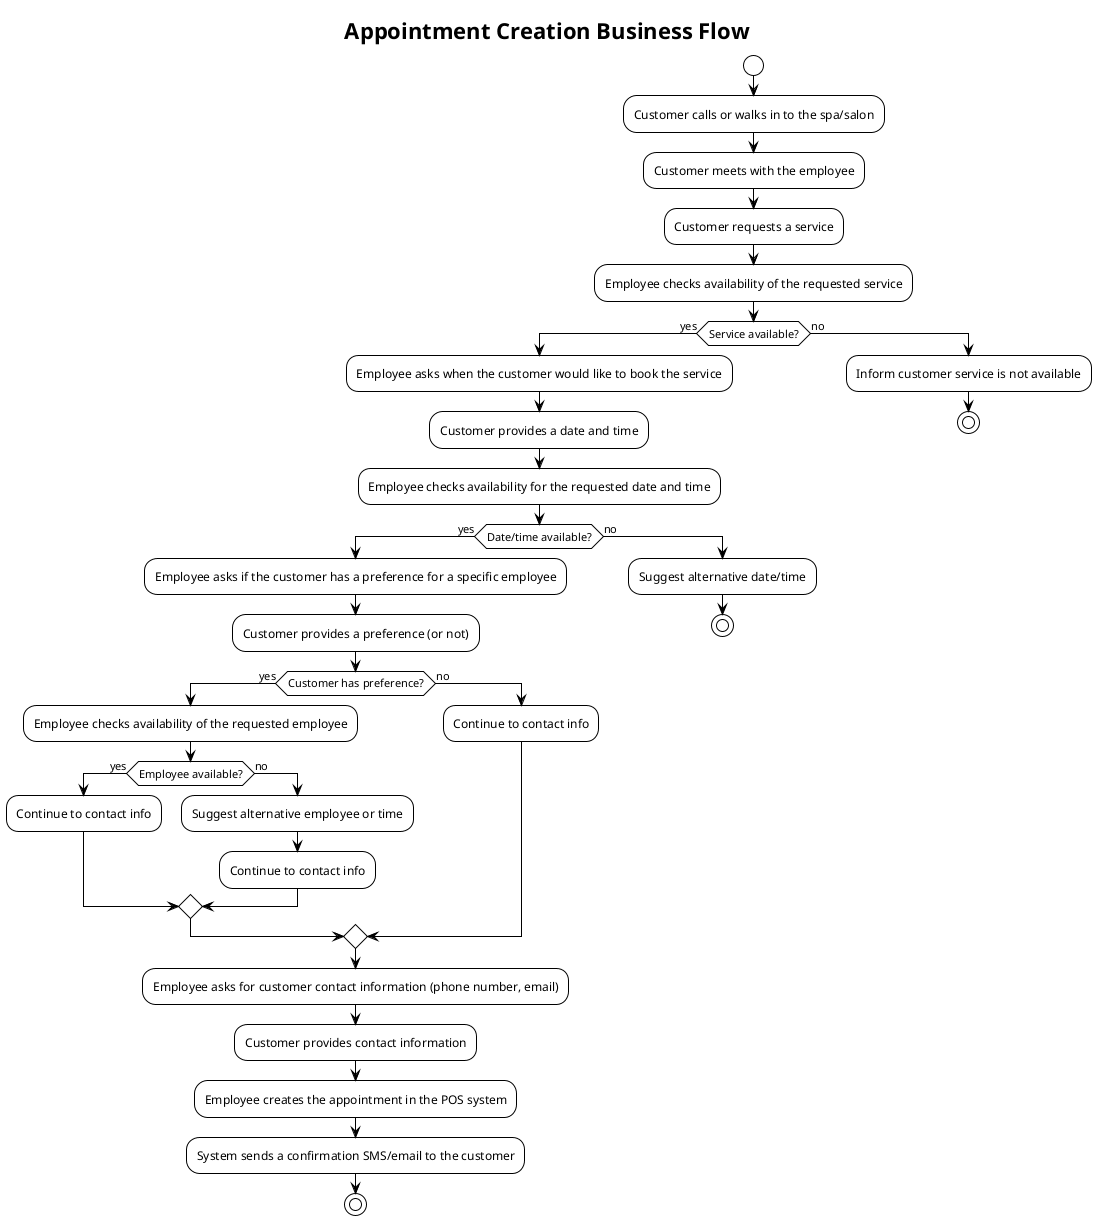
\includegraphics[width=0.8\textwidth]{images/diagrams/services/appointment_creation_flow.png}
    \caption{Appointment Creation Flow Diagram}
    \label{fig:appointment_creation_flow}
\end{figure}

\noticecomment{the suggest alternative employee or time needs to also include text that customer can opt for any available employee or time slot}

\suggestioncomment{Perhaps try to split this business flow into two different flows for the purpose of readability. Idea: two flows based on if date/time available}

\begin{figure}[H]
    \centering
    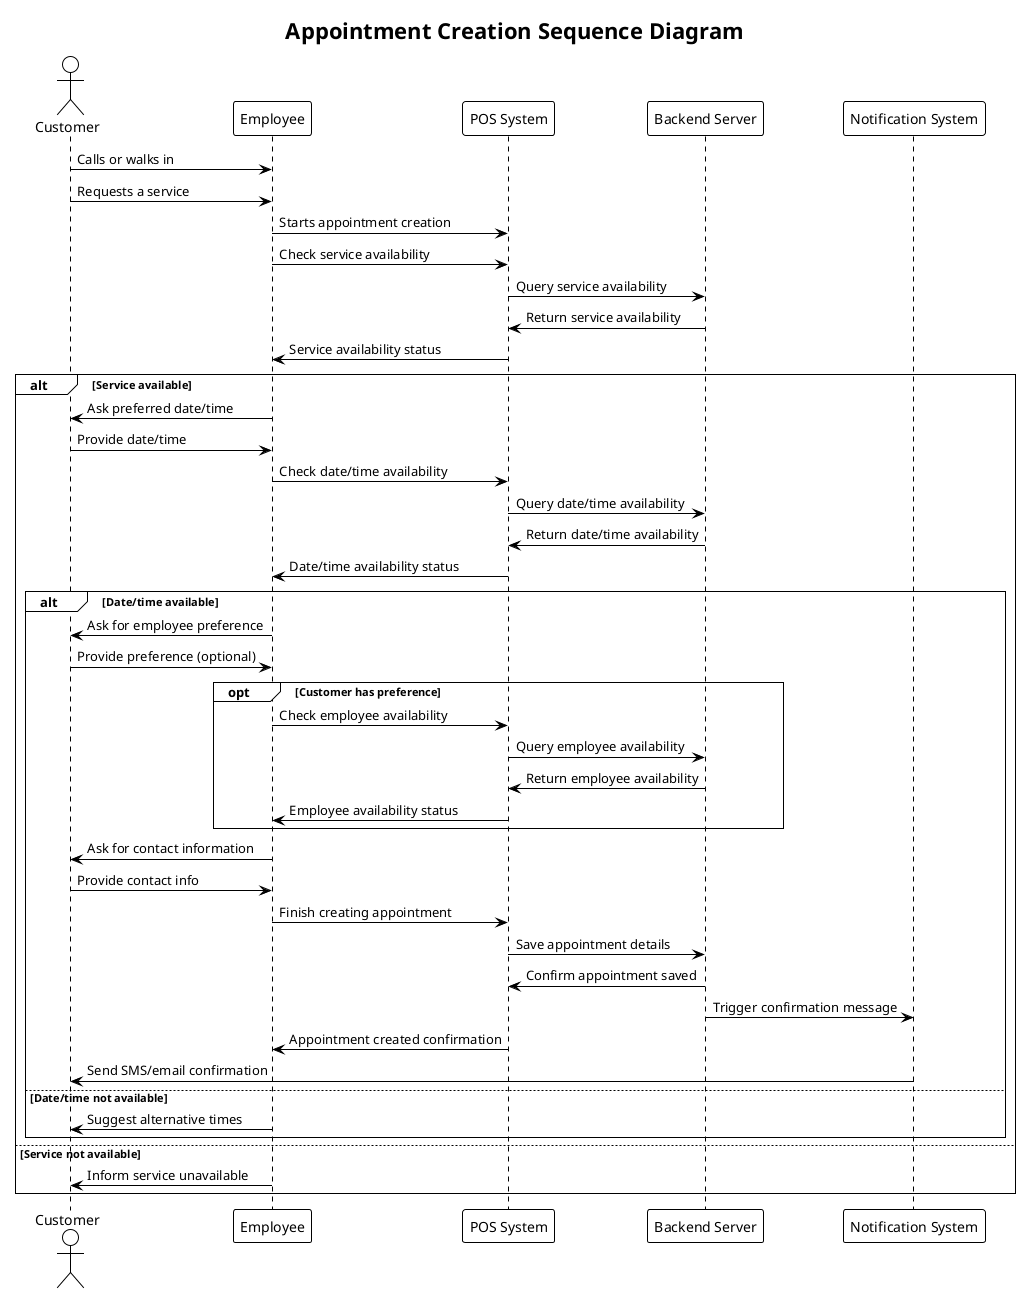
\includegraphics[width=0.8\textwidth]{images/diagrams/services/appointment_creation_sequence.png}
    \caption{Appointment Creation Sequence Diagram}
    \label{fig:appointment_creation_sequence}
\end{figure}

\subsubsection{Appointment modification business flow}

\textbf{BASIC FLOW:}

Customer calls or walks in to the spa/salon.
Customer meets with the employee.
Customer requests to modify an existing appointment.
Employee asks for customer contact information (phone number, email).
Customer provides contact information.
Employee retrieves the appointment using the provided contact information.
Employee discusses the requested changes with the customer (date, time, service, employee).
Employee checks availability for the requested changes.
If available, employee updates the appointment in the POS system.
System sends an updated confirmation SMS/email to the customer.

\textbf{ALTERNATIVE FLOW:}


\begin{itemize}
\item \textbf{No appointment found: } The employee cannot find an appointment matching the provided contact information.
Employee informs the customer that no appointment was found. 
\item \textbf{Slot taken: } The time slot or employee requested by the customer is not available.
Employee informs the customer of the unavailability and suggests alternative options.
Customer selects an alternative option.
\end{itemize}




\begin{center}
\setlength{\tabcolsep}{8pt}
\begin{tabular}{|p{0.48\linewidth}|p{0.48\linewidth}|}
\hline
\textbf{Tables/Entities} \newline
\begin{tabular}{@{}l@{}}
Customer \\
Employee \\
Service \\
Appointment \\
Spa/Salon (Business)
\end{tabular}
&
\textbf{Components} \newline
\begin{tabular}{@{}l@{}}
Appointment Management \\(Appointment, Employee, Service)  \\
Employee Management (Employee) \\
Notification System (SMS/Email)
\end{tabular}
\\ \hline
\textbf{Actions} \newline
\begin{tabular}{@{}l@{}}
Retrieve appointment \\
Check availability of service \\
Check availability of employee \\
Update appointment \\
Send updated confirmation notification
\end{tabular}
&
% \textbf{Notes} \newline
\begin{tabular}{@{}l@{}}
% \small Reserved for additional details or future items.
\end{tabular}
\\ \hline
\end{tabular}
\end{center}

\begin{figure}[H]
    \centering
    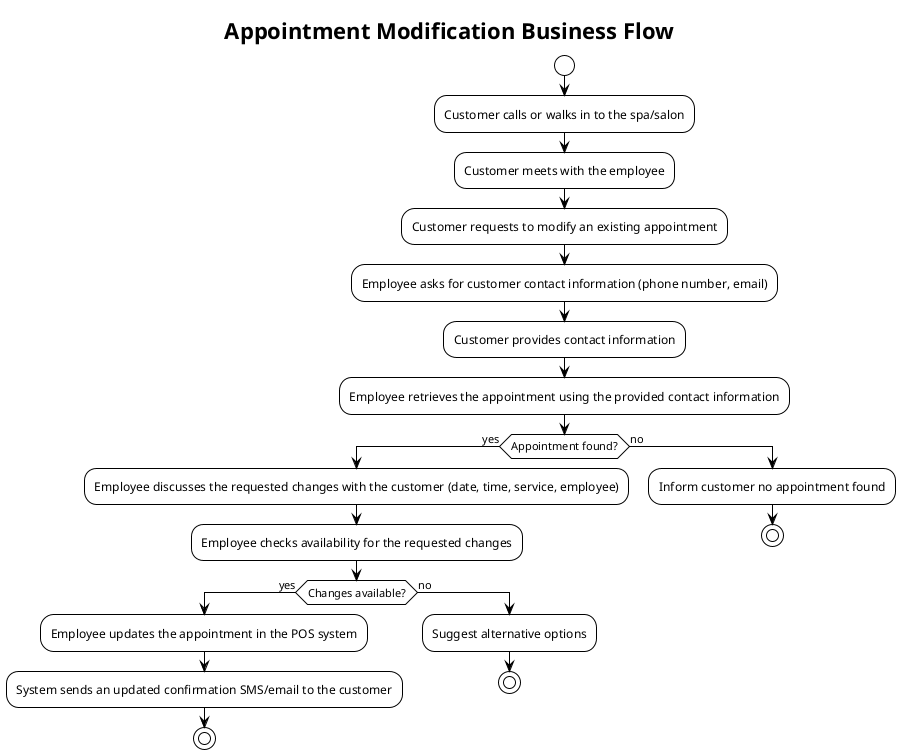
\includegraphics[width=0.8\textwidth]{images/diagrams/services/appointment_modification_flow.png}
    \caption{Appointment Modification Flow Diagram}
    \label{fig:appointment_modification_flow}
\end{figure}

\begin{figure}[H]
    \centering
    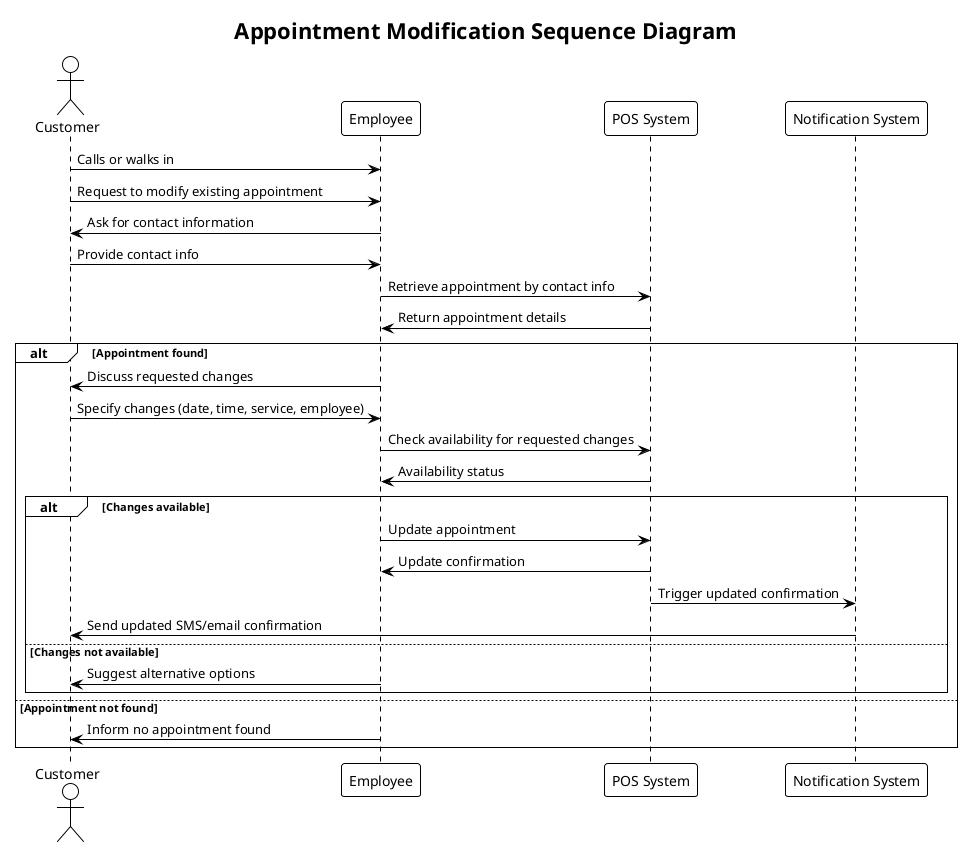
\includegraphics[width=0.8\textwidth]{images/diagrams/services/appointment_modification_sequence.png}
    \caption{Appointment Modification Sequence Diagram}
    \label{fig:appointment_modification_sequence}
\end{figure}

\subsubsection{Cancel appointment business flow}
\textbf{BASICL FLOW:}
Customer calls or walks in to the spa/salon.
Customer meets with the employee.
Customer requests to cancel an existing appointment.
Employee asks for customer contact information (phone number, email).
Customer provides contact information.
Employee retrieves the appointment using the provided contact information.
Employee confirms the cancellation with the customer.
Employee cancels the appointment in the POS system.
System sends a cancellation confirmation SMS/email to the customer.

\textbf{ALTERNATIVE FLOWS:}
\begin{itemize}
    \item \textbf{No appointment found: } The employee cannot find an appointment matching the provided contact information.
    Employee informs the customer that no appointment was found.
\end{itemize}


\begin{center}
\setlength{\tabcolsep}{8pt}
\begin{tabular}{|p{0.48\linewidth}|p{0.48\linewidth}|}
\hline
\textbf{Tables/Entities} \newline
\begin{tabular}{@{}l@{}}
Customer \\
Employee \\
Service \\
Appointment \\
Spa/Salon (Business)
\end{tabular}
&
\textbf{Components} \newline
\begin{tabular}{@{}l@{}}
Appointment Management \\ (Appointment, Employee, Service) \\
Employee Management (Employee) \\
Notification System (SMS/Email)
\end{tabular}
\\ \hline
\textbf{Actions} \newline
\begin{tabular}{@{}l@{}}
Retrieve appointment \\
Cancel appointment \\
Send cancellation confirmation notification
\end{tabular}
&
\begin{tabular}{@{}l@{}}
% \small Reserved for additional details or future items.
\end{tabular}
\\ \hline
\end{tabular}
\end{center}

\begin{figure}[H]
    \centering
    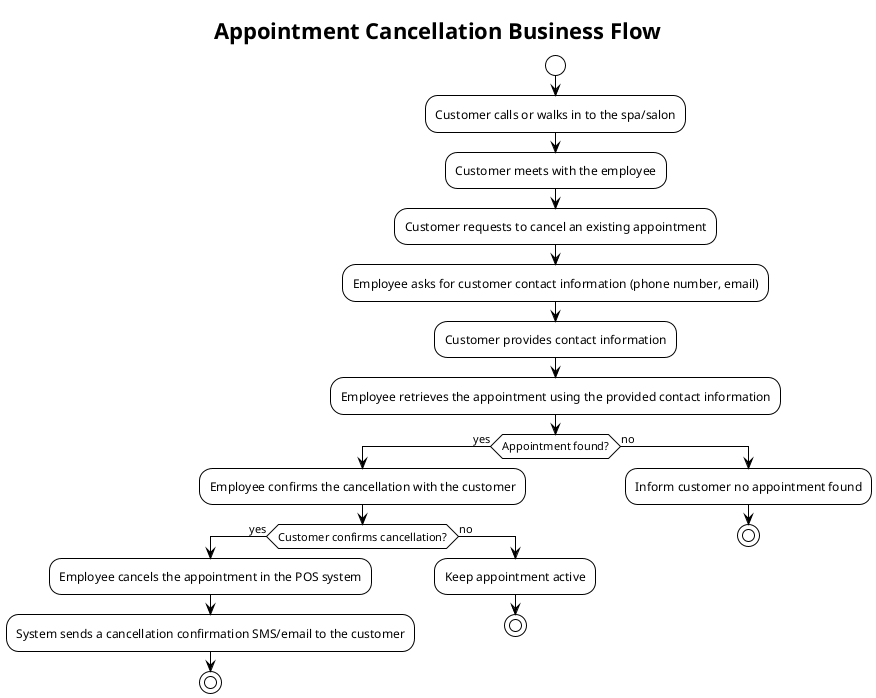
\includegraphics[width=0.8\textwidth]{images/diagrams/services/appointment_cancellation_flow.png}
    \caption{Appointment Cancellation Flow Diagram}
    \label{fig:appointment_cancellation_flow}
\end{figure}

\begin{figure}[H]
    \centering
    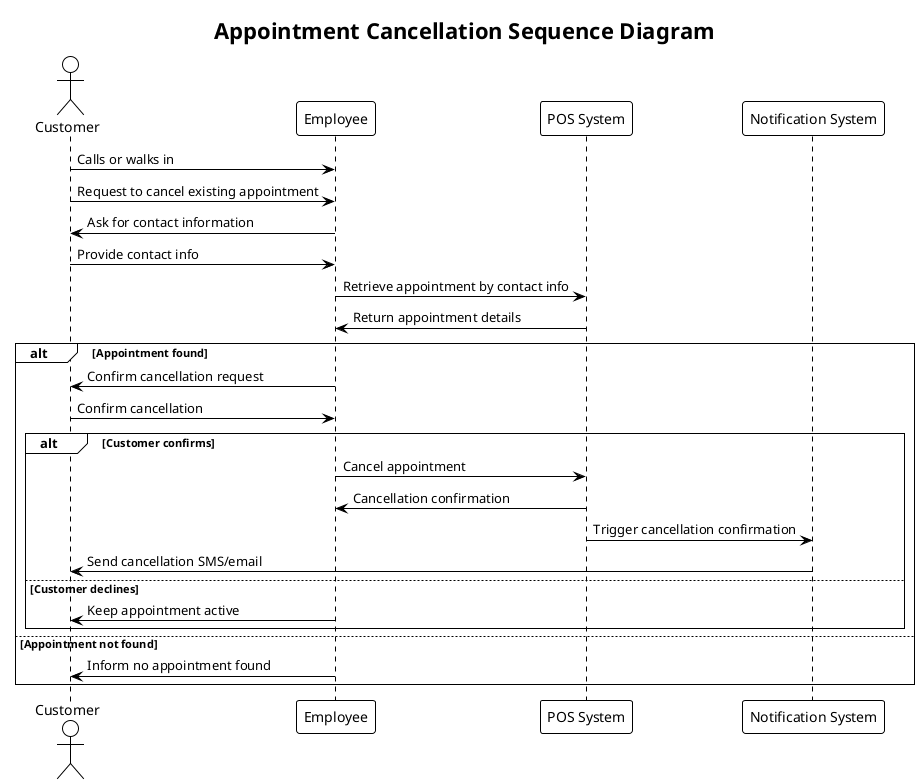
\includegraphics[width=0.8\textwidth]{images/diagrams/services/appointment_cancellation_sequence.png}
    \caption{Appointment Cancellation Sequence Diagram}
    \label{fig:appointment_cancellation_sequence}
\end{figure}

\subsubsection{Service customer business flow}

\textbf{BASIC FLOW:}

Customer arrives at the spa/salon for their scheduled appointment.
Employee greets the customer and asks customer to confirm their appointment details.
Employee verifies the appointment details in the POS system.
Employee directs the customer to the appropriate service area and employee.
Employee begins providing the scheduled service to the customer.
Employee completes the service according to the appointment specifications.
Employee asks the customer for the payment method.
Customer provides payment information (cash, card, etc.).
Employee processes the payment in the POS system.
System confirms payment and updates the appointment status.
Employee asks if the user would like a receipt.
If yes, employee prints or emails the receipt to the customer.
Customer departs.

\textbf{ALTERNATIVE FLOWS:}
\textbf{No appointment found: } The employee cannot find an appointment matching the provided contact information.
Employee informs the customer that no appointment was found.

\begin{center}
\setlength{\tabcolsep}{8pt}
\begin{tabular}{|p{0.48\linewidth}|p{0.48\linewidth}|}
\hline
\textbf{Tables/Entities} \newline
\begin{tabular}{@{}l@{}}
Customer \\
Employee \\
Service \\
Appointment \\
Payment \\
Spa/Salon (Business)
\end{tabular}
&
\textbf{Components} \newline
\begin{tabular}{@{}l@{}}
Appointment Management \\ (Appointment, Service) \\
Employee Management (Employee) \\
Payment Processing (Payment) \\
Notification System (Follow-up notifications)
\end{tabular}
\\ \hline
\textbf{Actions} \newline
\begin{tabular}{@{}l@{}}
Verify appointment details \\
Process payment \\
Mark service as completed \\
Generate receipt
\end{tabular}
&
\begin{tabular}{@{}l@{}}
% Reserved for additional notes or future items.
\end{tabular}
\\ \hline
\end{tabular}
\end{center}

\begin{figure}[H]
    \centering
    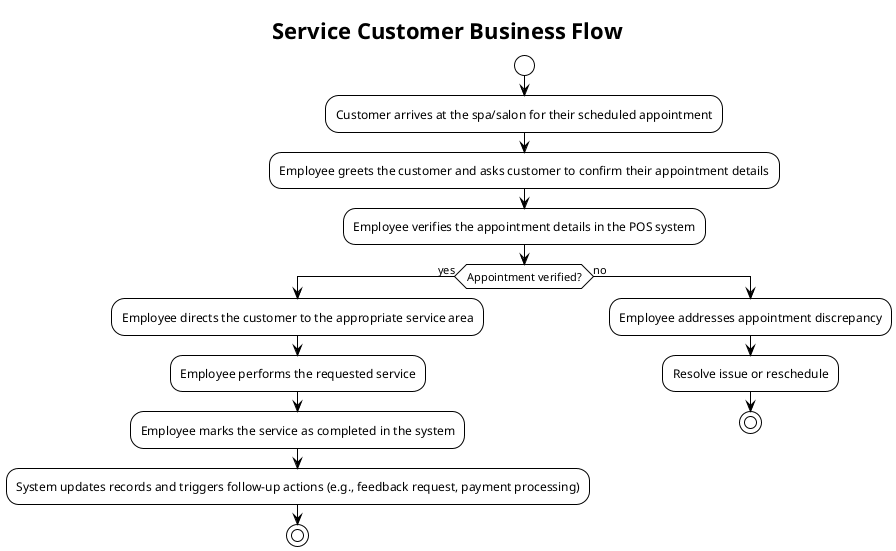
\includegraphics[width=0.8\textwidth]{images/diagrams/services/service_customer_flow.png}
    \caption{Service Customer Flow Diagram}
    \label{fig:service_customer_flow}
\end{figure}

\noticecomment{It says in the alternative flow employee addresses appointment discrepency, but in the flow it just says informs the customer. }

\begin{figure}[H]
    \centering
    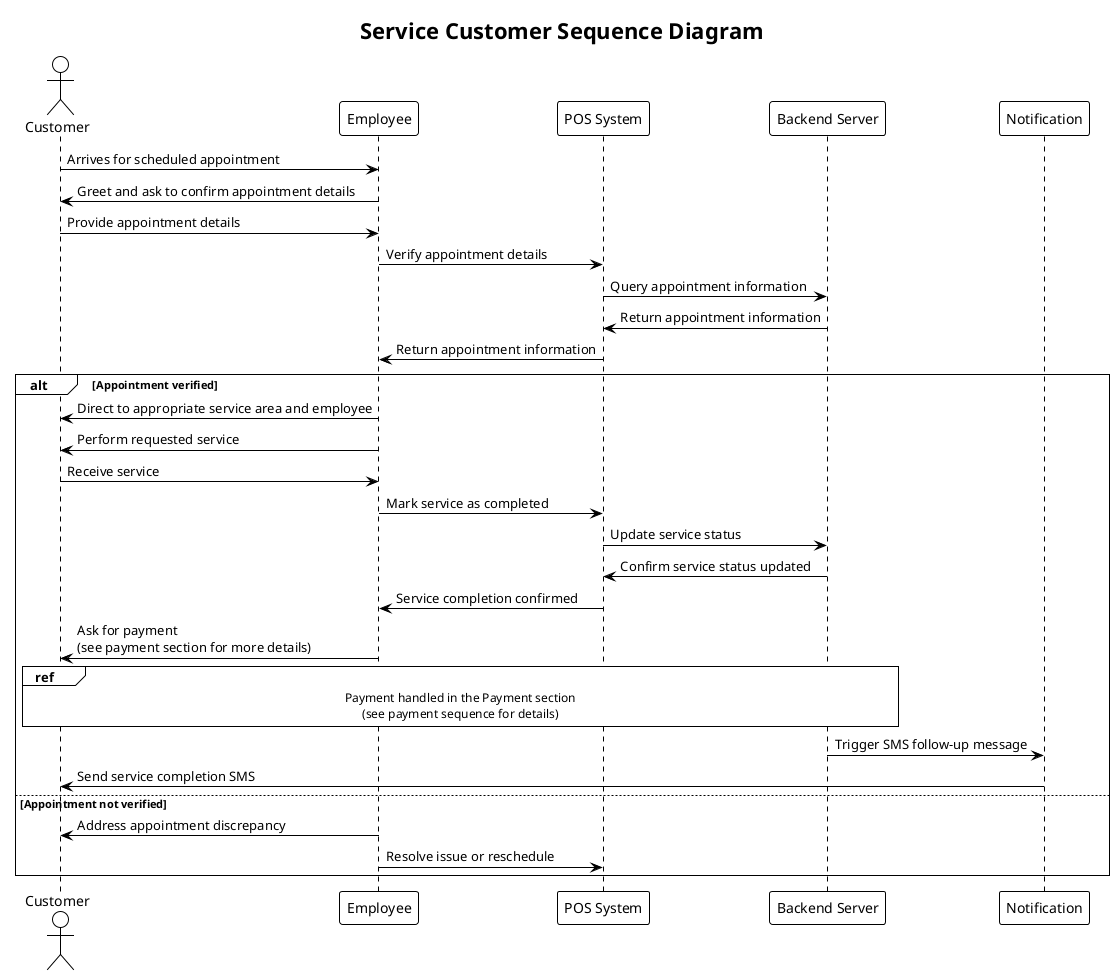
\includegraphics[width=0.8\textwidth]{images/diagrams/services/service_customer_sequence.png}
    \caption{Service Customer Sequence Diagram}
    \label{fig:service_customer_sequence}
\end{figure}

\subsection{Payment}

\subsubsection{Supported Payment Methods}
\begin{itemize}
\item Cash
\item Gift card
\item Credit/debit card (via Stripe)
\end{itemize}

\subsubsection{Key Business Rules}
\begin{itemize}
\item Split payments are supported: an order total can be paid by multiple parties and/or multiple payment methods.
\item Employees can add tips and apply discounts during payment.
\item Final receipts must include applicable taxes, tips, and discounts for each payment.
\item Closed/paid orders are preserved for audit purposes and can be refunded (partial or total).
\item Refund for card payments is processed through Stripe. For other methods, the status is updated in the system.
\end{itemize}

\subsubsection{Payment Flow}
The following sequence diagram illustrates the payment process, including split payments, tips, and refunds.

\begin{figure}[H]
    \centering
    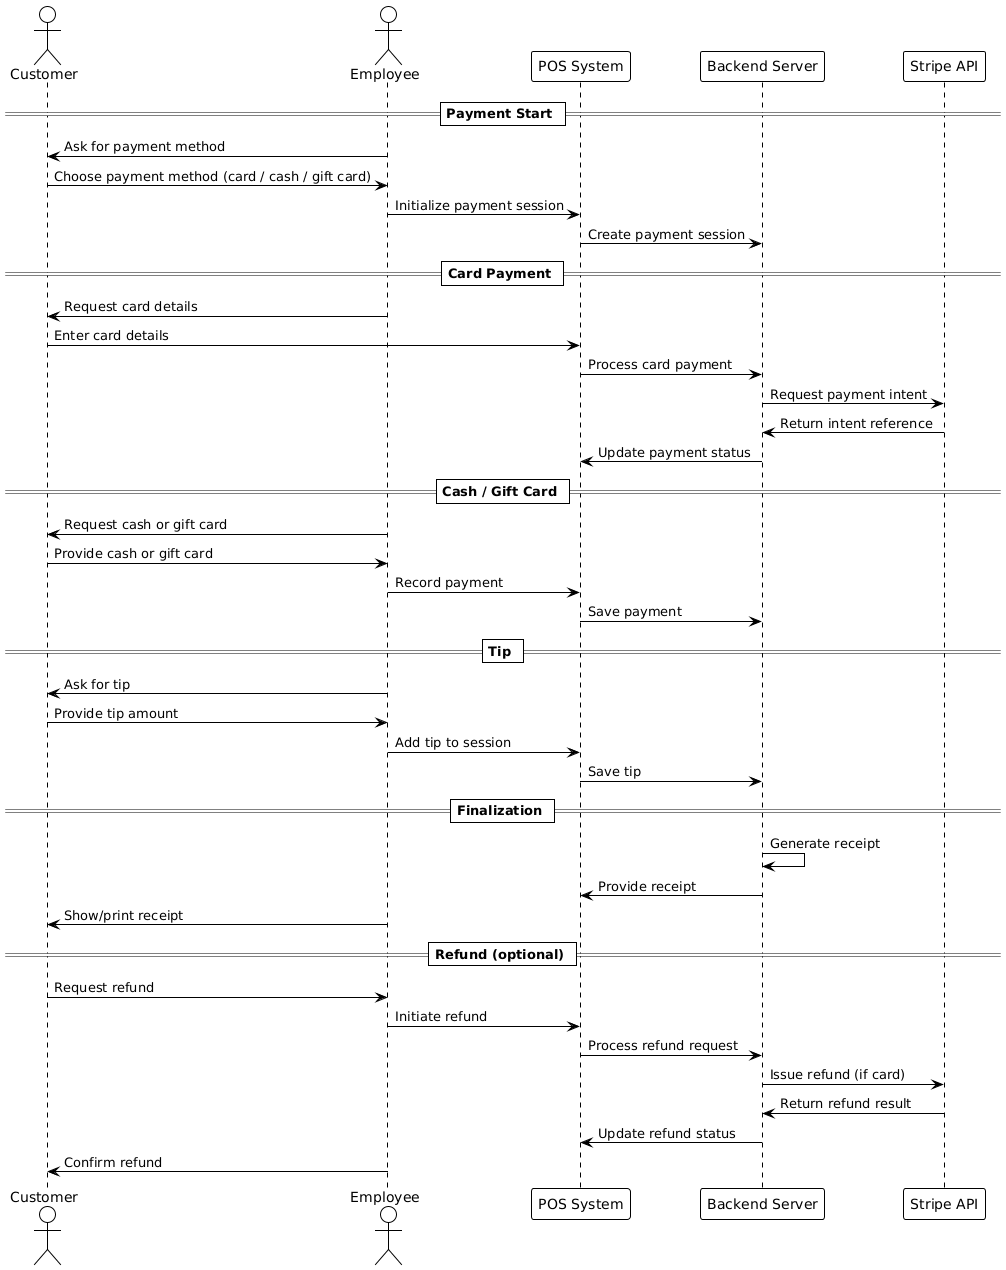
\includegraphics[width=1\textwidth]{docs/ps-design/design-document/images/diagrams/payment/payment_flow.png}
    \caption{Payment Flow Sequence Diagram}
    \label{fig:payment_flow}
\end{figure}

\subsection{Business Management}


% ------------------------------------------------------------------------
% MANAGEMENT DOMAIN (System-wide administrative and operational functions)
% ------------------------------------------------------------------------
% Use Case                           | Description
% ------------------------------------------------------------------------
% User Management                    | Specify business owner can only edit their business's users
% Manage Products/Services           | Add, edit, or deactivate products or services (e.g., menu items, massage types). 
% Manage Product Variations          | Create/edit modifiers for products (e.g., milk type, decaf, size)
% Manage Employees                   | Create, update, or deactivate employee accounts.
% Manage Business Info               | Update business details (owner, address, name, tax ID, contact info).
% Manage Inventory (Optional)        | Track stock levels of items (e.g., ingredients, products).
% Manage Taxes                       | Configure tax rates (e.g., VAT) for different products or services.
% Manage Users & Roles               | Assign permissions to employees (e.g., manager, cashier, admin).
% Super Admin Access                 | Special user (system operator) can access all businesses for support.
% View Reports                       | Generate reports on orders, appointments, revenue, etc.
% Manage Modifiers/Variants          | Define product variants (e.g., latte with almond milk, decaf).
% Manage Discounts                   | Create and manage discount rules (e.g., seasonal, loyalty).
% Manage Service Charges/Tips        | Manage Service Charges/Tips	Configure service charge/gratuity rules (change shouldn't affect historical records)
% Time-Limited Discounts             | Create discounts that are valid only for specific time periods
% ------------------------------------------------------------------------


% ------------------------------------------------------------------------
% Cross-Domain Use Cases (Apply to multiple domains)
% ------------------------------------------------------------------------
% | Use Case                 | Description                                             
% |--------------------------|---------------------------------------------------------
% | Login / Authentication   | Employees log into the system.                          
% | Logout                   | Secure session end.                                     
% | View History             | View past orders or appointments.                       
% | Historical Data Consistency Check   | Ensure changes (e.g., tax updates) don’t affect         
% |                                     | historical records.                                     
% ------------------------------------------------------------------------
We have identified the following Use cases for the Business management domain:

\vspace{1cm}
\begin{longtable}{p{0.25\linewidth} p{0.70\linewidth}}
\caption{Use cases for the Business Management domain} \\
\textbf{Use case} & \textbf{Description} \\
\hline
\endfirsthead

\multicolumn{2}{c}{{\tablename\ \thetable{} -- Continued from previous page}} \\
\textbf{Use case} & \textbf{Description} \\
\hline
\endhead

\multicolumn{2}{c}{{Continued on next page}} \\
\endfoot

\endlastfoot

User Management &
\begin{minipage}[t]{\linewidth}
The business owner can create, update, or deactivate users within their own business. They cannot modify accounts belonging to other businesses.
\end{minipage} \\[6pt]
\multicolumn{2}{@{}c@{}}{\color{gray}\rule{0.95\linewidth}{0.4pt}} \\[6pt]
Manage Products \\ and Services &
\begin{minipage}[t]{\linewidth}
The business owner or authorized staff can add new products/services, edit details (name, price, category), or deactivate them (e.g., coffee, massage type).
\end{minipage} \\[6pt]
\multicolumn{2}{@{}c@{}}{\color{gray}\rule{0.95\linewidth}{0.4pt}} \\[6pt]
Manage Product Variations &
\begin{minipage}[t]{\linewidth}
The business owner or staff can define or edit product modifiers, such as size (small/medium/large), add-ons or other options.
\end{minipage} \\[6pt]
\multicolumn{2}{@{}c@{}}{\color{gray}\rule{0.95\linewidth}{0.4pt}} \\[6pt]
Manage Employees &
\begin{minipage}[t]{\linewidth}
The business owner can create new employee accounts, update employee details (role, contact, availability), or deactivate accounts.
\end{minipage} \\[6pt]
\multicolumn{2}{@{}c@{}}{\color{gray}\rule{0.95\linewidth}{0.4pt}} \\[6pt]
Manage Business Info &
\begin{minipage}[t]{\linewidth}
The business owner can update business details such as the name, address, tax ID, contact information, or ownership information.
\end{minipage} \\[6pt]
\multicolumn{2}{@{}c@{}}{\color{gray}\rule{0.95\linewidth}{0.4pt}} \\[6pt]
Manage Inventory (Optional) &
\begin{minipage}[t]{\linewidth}
The business can track and update stock levels of ingredients or products. System automatically reduces inventory when items are sold, and can alert when stock is low.
\end{minipage} \\[6pt]
\multicolumn{2}{@{}c@{}}{\color{gray}\rule{0.95\linewidth}{0.4pt}} \\[6pt]
Manage Taxes &
\begin{minipage}[t]{\linewidth}
Admins can configure tax rules and rates (e.g., VAT, sales tax) for products or services. Updates affect only new transactions; historical data remains unchanged.
\end{minipage} \\[6pt]
\multicolumn{2}{@{}c@{}}{\color{gray}\rule{0.95\linewidth}{0.4pt}} \\[6pt]
Manage Users \\ and Roles &
\begin{minipage}[t]{\linewidth}
The business owner can assign system roles (manager, cashier, admin, etc.) to employees, controlling access rights and permissions within the system.
\end{minipage} \\[6pt]
\multicolumn{2}{@{}c@{}}{\color{gray}\rule{0.95\linewidth}{0.4pt}} \\[6pt]
Super Admin Access &
\begin{minipage}[t]{\linewidth}
A system operator (Super Admin) can access any business account in the system for technical support, troubleshooting, or emergency fixes.
\end{minipage} \\[6pt]
\multicolumn{2}{@{}c@{}}{\color{gray}\rule{0.95\linewidth}{0.4pt}} \\[6pt]
Manage Modifiers/Variants &
\begin{minipage}[t]{\linewidth}
Admin can define product variants such as “latte with almond milk” or “spa service with aromatherapy add-on.” Variants allow customer customization at order time.
\end{minipage} \\[6pt]
\multicolumn{2}{@{}c@{}}{\color{gray}\rule{0.95\linewidth}{0.4pt}} \\[6pt]
Manage Discounts &
\begin{minipage}[t]{\linewidth}
Admins can create and manage discount rules (percentage-based, fixed amount, seasonal campaigns, loyalty discounts).
\end{minipage} \\[6pt]
\multicolumn{2}{@{}c@{}}{\color{gray}\rule{0.95\linewidth}{0.4pt}} \\[6pt]
Manage Service Charges/Tips &
\begin{minipage}[t]{\linewidth}
Admins can configure rules for applying service charges or gratuities. Updates only apply to future transactions, ensuring historical data remains intact.
\end{minipage} \\[6pt]
\multicolumn{2}{@{}c@{}}{\color{gray}\rule{0.95\linewidth}{0.4pt}} \\[6pt]
Time-Limited Discounts &
\begin{minipage}[t]{\linewidth}
Admins can create discounts restricted to a specific timeframe (e.g., happy hour, seasonal promotions). The system enforces validity automatically.
\end{minipage} \\[6pt]
\multicolumn{2}{@{}c@{}}{\color{gray}\rule{0.95\linewidth}{0.4pt}} \\[6pt]

\end{longtable}

We have identified the following Cross-Domain Use cases for the Business management domain:
\vspace{1cm}
\begin{longtable}{p{0.25\linewidth} p{0.70\linewidth}}
\caption{Cross-Domain Use cases for the Business Management domain} \\
\textbf{Use case} & \textbf{Description} \\
\hline
\endfirsthead

\multicolumn{2}{c}{{\tablename\ \thetable{} -- Continued from previous page}} \\
\textbf{Use case} & \textbf{Description} \\
\hline
\endhead

\multicolumn{2}{c}{{Continued on next page}} \\
\endfoot

\endlastfoot

Login / Authentication &
\begin{minipage}[t]{\linewidth}
Employees log into the system using their credentials. The system validates identity and assigns permissions based on role.
\end{minipage} \\[6pt]
\multicolumn{2}{@{}c@{}}{\color{gray}\rule{0.95\linewidth}{0.4pt}} \\[6pt]
Logout &
\begin{minipage}[t]{\linewidth}
Employees securely end their session. The system clears active tokens/sessions and confirms logout Users (customers, employees, or admins) can view past orders, appointments, or reports. This ensures transparency and auditability.
\end{minipage} \\[6pt]
\multicolumn{2}{@{}c@{}}{\color{gray}\rule{0.95\linewidth}{0.4pt}} \\[6pt]
View Historical Data, Consistency Check &
\begin{minipage}[t]{\linewidth}
Users (customers, employees, or admins) can view past orders, appointments, or reports. This ensures transparency and auditability.
\end{minipage} \\[6pt]
\multicolumn{2}{@{}c@{}}{\color{gray}\rule{0.95\linewidth}{0.4pt}} \\[6pt]
Historical Data Consistency Check &
\begin{minipage}[t]{\linewidth}
The system ensures that administrative changes (tax rates, discounts, service charges) apply only to new transactions, without modifying historical order or appointment records.
\end{minipage} \\[6pt]
\multicolumn{2}{@{}c@{}}{\color{gray}\rule{0.95\linewidth}{0.4pt}} \\[6pt]

\end{longtable}
% related use cases: User Management, Manage Employees, Manage Users & Roles, Super Admin Access

\newpage
\subsubsection{User Management Business Flow}

Flow:
\begin{itemize}
\setlength{\itemsep}{2pt}
\setlength{\parskip}{0pt}
\setlength{\parsep}{0pt}
\item Owner logs into the system and navigates to the User Management section.
\item Owner chooses an action: create new user, update existing user, or deactivate a user.
\item System prompts for user details (name, email, role, business association, status).
\item Owner provides or modifies the required details.
\item System invokes the Auth Service to validate that the owner can only manage users of their own business.
\item If validation passes, system executes the requested operation through the User Service:
\begin{itemize}
\item Create user → insert new record into User Table.
\item Update user → modify existing record in User Table.
\item Deactivate user → mark record as inactive (soft delete).
\end{itemize}
\item System commits changes to the database.
\item System confirms the operation result to the owner (success or failure).
\end{itemize}

Tables/Entities:
\begin{itemize}
\setlength{\itemsep}{2pt}
\setlength{\parskip}{0pt}
\setlength{\parsep}{0pt}
\item Owner (Business Owner)
\item User (employee or other system user tied to the business)
\item Business (reference to ensure ownership validation)
\item User Table (stores user records, roles, status)
\item Auth Session (validates logged-in identity and permissions)
\end{itemize}

Components:
\begin{itemize}
\setlength{\itemsep}{2pt}
\setlength{\parskip}{0pt}
\setlength{\parsep}{0pt}
\item User Interface (forms for inputting user details, displaying results)
\item Auth Service (validates business ownership and permissions)
\item User Service (handles create, update, deactivate logic)
\item Database Layer (User Table persistence)
\end{itemize}

Actions:
\begin{itemize}
\setlength{\itemsep}{2pt}
\setlength{\parskip}{0pt}
\setlength{\parsep}{0pt}
\item Navigate to User Management
\item Select user action (create / update / deactivate)
\item Input or edit user details
\item Validate ownership and permissions
\item Execute database transaction (insert / update / deactivate record)
\item Confirm operation result to owner
\end{itemize}

\begin{figure}[H]
    \centering
    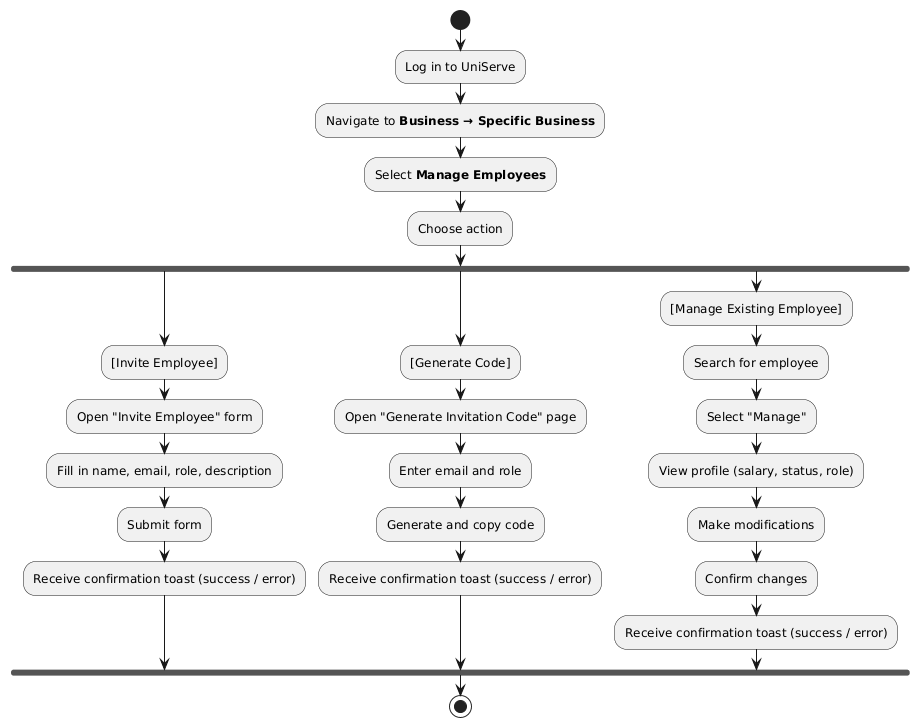
\includegraphics[width=1\textwidth]{images/diagrams/business/bpmn_user_manage.png}
    \caption{User Management Business Flow Diagram}
    \label{fig:user_manage_flow}
\end{figure}

\subsubsection{Manage Products/Services Business Flow}

Flow:
\begin{itemize}
\setlength{\itemsep}{2pt}
\setlength{\parskip}{0pt}
\setlength{\parsep}{0pt}
\item Owner logs into the system and navigates to the Manage Products/Services section.
\item Owner chooses an action: create new product/service, update details of an existing product/service, or deactivate an item.
\item System prompts for product/service details (name, description, price, category, status).
\item Owner provides or modifies the required details.
\item System invokes the Auth Service to validate that the owner is authorized to manage only their business’s items.
\item If validation passes, system executes the requested operation through the Product/Service Service:
\begin{itemize}
\item Create product/service → insert new record into Product/Service Table.
\item Update product/service → modify existing record in Product/Service Table.
\item Deactivate product/service → mark record as inactive (soft delete).
\end{itemize}
\item System commits changes to the database.
\item System confirms the operation result to the owner (success or failure).
\end{itemize}

Tables/Entities:
\begin{itemize}
\setlength{\itemsep}{2pt}
\setlength{\parskip}{0pt}
\setlength{\parsep}{0pt}
\item Owner (Business Owner / Manager)
\item Product/Service (the item being managed)
\item Business (reference to ensure ownership validation)
\item Product/Service Table (stores product/service records, categories, price, status)
\item Auth Session (validates logged-in identity and permissions)
\end{itemize}

Components:
\begin{itemize}
\setlength{\itemsep}{2pt}
\setlength{\parskip}{0pt}
\setlength{\parsep}{0pt}
\item User Interface (forms for product/service details, status changes)
\item Auth Service (validates ownership and permissions)
\item Product/Service Service (handles CRUD logic for products/services)
\item Database Layer (Product/Service Table persistence)
\end{itemize}

Actions:
\begin{itemize}
\setlength{\itemsep}{2pt}
\setlength{\parskip}{0pt}
\setlength{\parsep}{0pt}
\item Navigate to Manage Products/Services
\item Select item action (create / update / deactivate)
\item Input or edit product/service details
\item Validate ownership and permissions
\item Execute database transaction (insert / update / deactivate record)
\item Confirm operation result to owner
\end{itemize}

\begin{figure}[H]
    \centering
    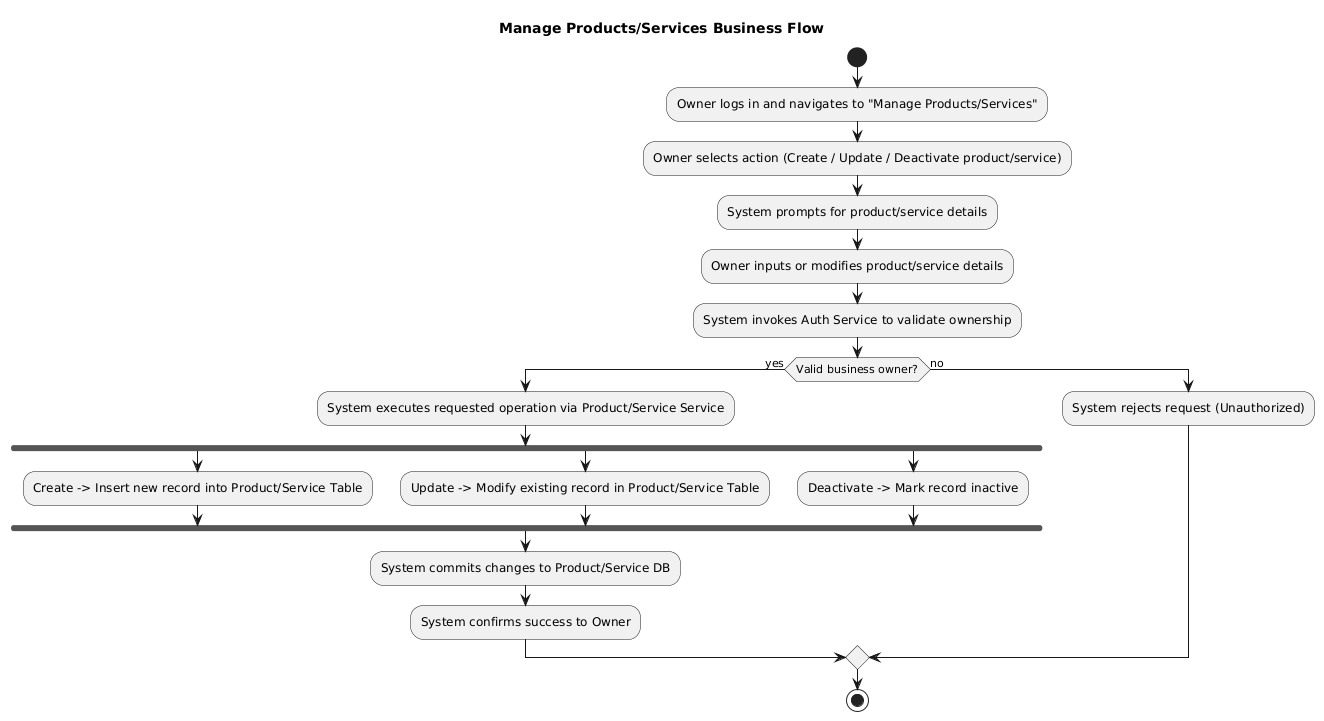
\includegraphics[width=1\textwidth]{images/diagrams/business/bpmn_products_services.png}
    \caption{Manage Products/Services Business Flow Diagram}
    \label{fig:product_service_manage_flow}
\end{figure}

\subsubsection{Manage Product Variations Business Flow}

Flow:
\begin{itemize}
\setlength{\itemsep}{2pt}
\setlength{\parskip}{0pt}
\setlength{\parsep}{0pt}
\item Owner or authorized staff logs into the system and navigates to the Manage Product Variations section.
\item Owner/staff selects an action: create new variation, update an existing variation, or delete/deactivate a variation.
\item System prompts for variation details (name, type, category, associated product, status).
\item Owner/staff provides or modifies variation details (e.g., size: small/medium/large; milk type: soy, almond; add-on: extra shot).
\item System invokes the Auth Service to validate permissions and business ownership.
\item If validation passes, system executes the requested operation through the Product Variation Service:
\begin{itemize}
\item Create variation → insert new record into Variation Table linked to a product.
\item Update variation → modify existing record in Variation Table.
\item Deactivate variation → mark record as inactive (soft delete).
\end{itemize}
\item System commits changes to the database.
\item System confirms the operation result to the owner/staff (success or failure).
\end{itemize}

Tables/Entities:
\begin{itemize}
\setlength{\itemsep}{2pt}
\setlength{\parskip}{0pt}
\setlength{\parsep}{0pt}
\item Owner/Staff (business users with permissions)
\item Product (base product associated with the variation)
\item Product Variation (modifiers/options for the product)
\item Business (reference for ownership validation)
\item Product Variation Table (stores variation details, product linkage, status)
\item Auth Session (validates user identity and role)
\end{itemize}

Components:
\begin{itemize}
\setlength{\itemsep}{2pt}
\setlength{\parskip}{0pt}
\setlength{\parsep}{0pt}
\item User Interface (variation forms: add/edit/remove options)
\item Auth Service (validates ownership and role permissions)
\item Product Variation Service (CRUD operations for variations/modifiers)
\item Database Layer (Variation Table persistence, product linkage)
\end{itemize}

Actions:
\begin{itemize}
\setlength{\itemsep}{2pt}
\setlength{\parskip}{0pt}
\setlength{\parsep}{0pt}
\item Navigate to Manage Product Variations
\item Select variation action (create / update / deactivate)
\item Input or edit variation details
\item Validate ownership and permissions
\item Execute database transaction (insert / update / deactivate variation)
\item Confirm operation result to owner/staff
\end{itemize}

\begin{figure}[H]
    \centering
    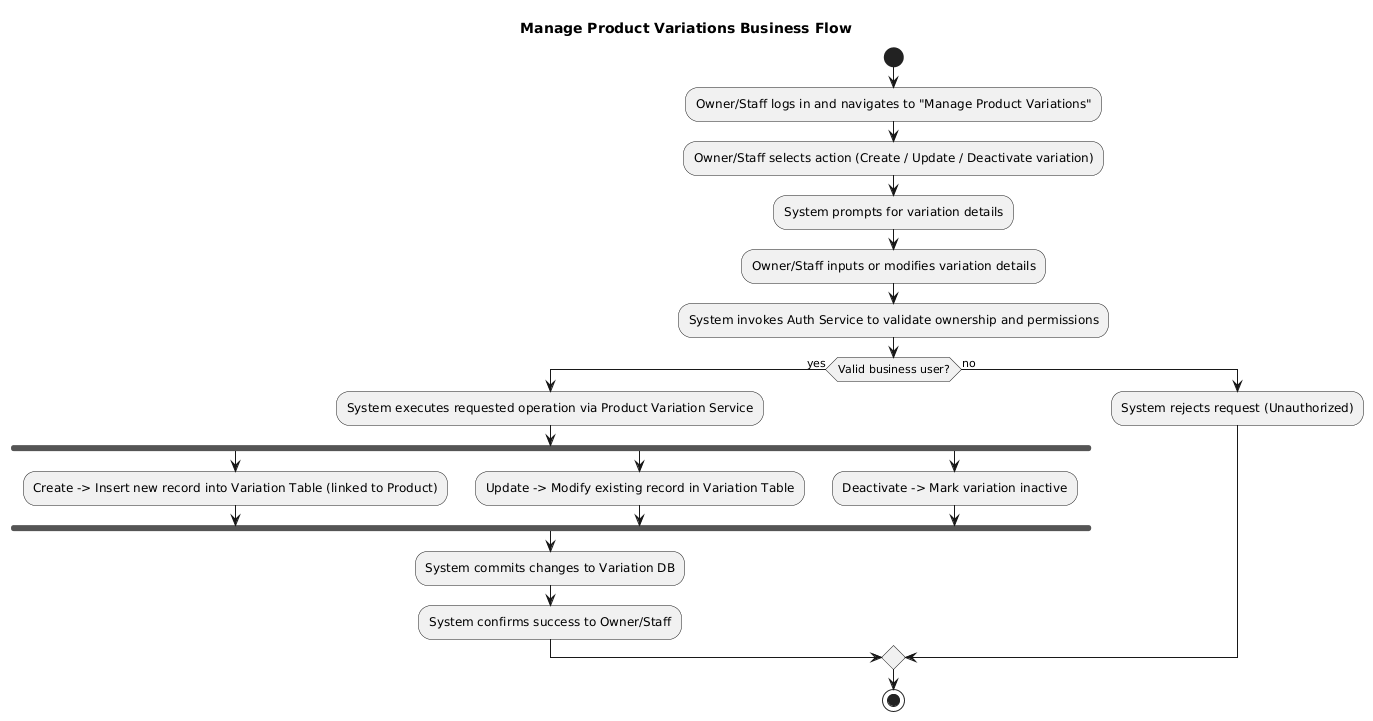
\includegraphics[width=1\textwidth]{images/diagrams/business/bpmn_product_variations.png}
    \caption{Manage Product Variations Business Flow Diagram}
    \label{fig:product_variations_manage_flow}
\end{figure}

\subsubsection{Manage Employees Business Flow}
Flow:
\begin{itemize}
\setlength{\itemsep}{2pt}
\setlength{\parskip}{0pt}
\setlength{\parsep}{0pt}
\item Owner logs into the system and navigates to the Manage Employees section.
\item Owner chooses an action: create new employee, update existing employee details, or deactivate an employee account.
\item System prompts for employee details (name, email, role, contact info, status).
\item Owner provides or modifies the required details.
\item System invokes the Auth Service to validate that the owner can only manage employees of their own
business.
\item If validation passes, system executes the requested operation through the Employee Service:
\begin{itemize}
\item Create employee → insert new record into Employee Table.
\item Update employee → modify existing record in Employee Table.
\item Deactivate employee → mark record as inactive (soft delete).
\end{itemize}
\item System commits changes to the database.
\item System confirms the operation result to the owner (success or failure).
\end{itemize}
Tables/Entities:
\begin{itemize}
\setlength{\itemsep}{2pt}
\setlength{\parskip}{0pt}
\setlength{\parsep}{0pt}
\item Owner (Business Owner)
\item Employee (the staff member being managed)
\item Business (reference to ensure ownership validation)
\item Employee Table (stores employee records, roles, status)
\item Auth Session (validates logged-in identity and permissions)
\end{itemize}
Components:
\begin{itemize}
\setlength{\itemsep}{2pt}
\setlength{\parskip}{0pt}
\setlength{\parsep}{0pt}
\item User Interface (forms for inputting employee details, displaying results)
\item Auth Service (validates business ownership and permissions)
\item Employee Service (handles create, update, deactivate logic)
\item Database Layer (Employee Table persistence)
\end{itemize}
Actions:
\begin{itemize}
\setlength{\itemsep}{2pt}
\setlength{\parskip}{0pt}
\setlength{\parsep}{0pt}
\item Navigate to Manage Employees
\item Select employee action (create / update / deactivate)
\item Input or edit employee details
\item Validate ownership and permissions
\item Execute database transaction (insert / update / deactivate record)
\item Confirm operation result to owner
\end{itemize}
\begin{figure}[H]
    \centering
    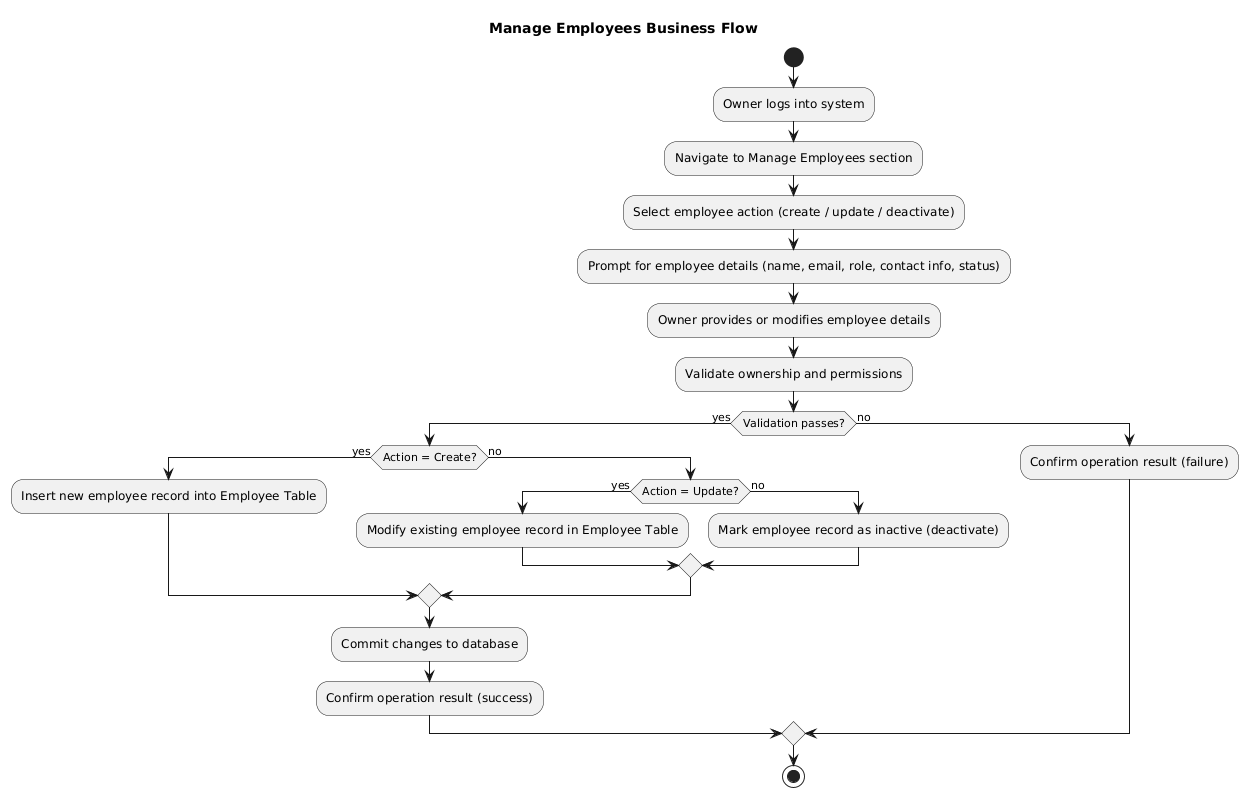
\includegraphics[width=1\textwidth]{images/diagrams/business/bpmn_employee_manage.png}
    \caption{Manage Employees Business Flow Diagram}
    \label{fig:employee_manage_flow}
\end{figure}

\subsubsection{Manage Business Info Business Flow}

Flow:
\begin{itemize}
    \setlength{\itemsep}{2pt}
    \setlength{\parskip}{0pt}
    \setlength{\parsep}{0pt}
    \item Owner logs into the system and navigates to the Business Info section.
    \item Owner selects an action: update business name, address, tax ID, contact information, or ownership details.
    \item System displays current business information and prompts for changes.
    \item Owner edits the desired fields and submits the update.
    \item System invokes the Auth Service to validate that the owner is authorized to modify only their own business.
    \item If validation passes, system updates the Business Table with the new information.
    \item System commits changes to the database.
    \item System confirms the operation result to the owner (success or failure).
\end{itemize}

Tables/Entities:
\begin{itemize}
    \setlength{\itemsep}{2pt}
    \setlength{\parskip}{0pt}
    \setlength{\parsep}{0pt}
    \item Owner (Business Owner)
    \item Business (stores business details)
    \item Business Table (name, address, tax ID, contact info, owner)
    \item Auth Session (validates logged-in identity and permissions)
\end{itemize}

Components:
\begin{itemize}
    \setlength{\itemsep}{2pt}
    \setlength{\parskip}{0pt}
    \setlength{\parsep}{0pt}
    \item User Interface (forms for editing business info)
    \item Auth Service (validates ownership and permissions)
    \item Business Service (handles update logic)
    \item Database Layer (Business Table persistence)
\end{itemize}

Actions:
\begin{itemize}
    \setlength{\itemsep}{2pt}
    \setlength{\parskip}{0pt}
    \setlength{\parsep}{0pt}
    \item Navigate to Business Info section
    \item Select info to update (name, address, tax ID, contact, owner)
    \item Edit and submit changes
    \item Validate ownership and permissions
    \item Execute database transaction (update business record)
    \item Confirm operation result to owner
\end{itemize}

\begin{figure}[H]
    \centering
    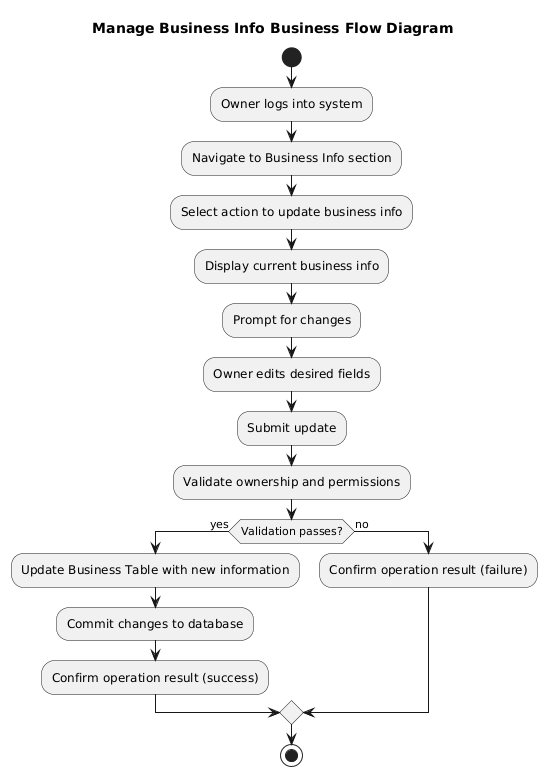
\includegraphics[width=0.6\textwidth]{images/diagrams/business/bpmn_business_info_manage.png}
    \caption{Manage Business Info Business Flow Diagram}
    \label{fig:business_info_manage_flow}
\end{figure}

\subsection{Data Model}

\subsubsection{Order Data Model}
\begin{figure}[H]
    \centering
    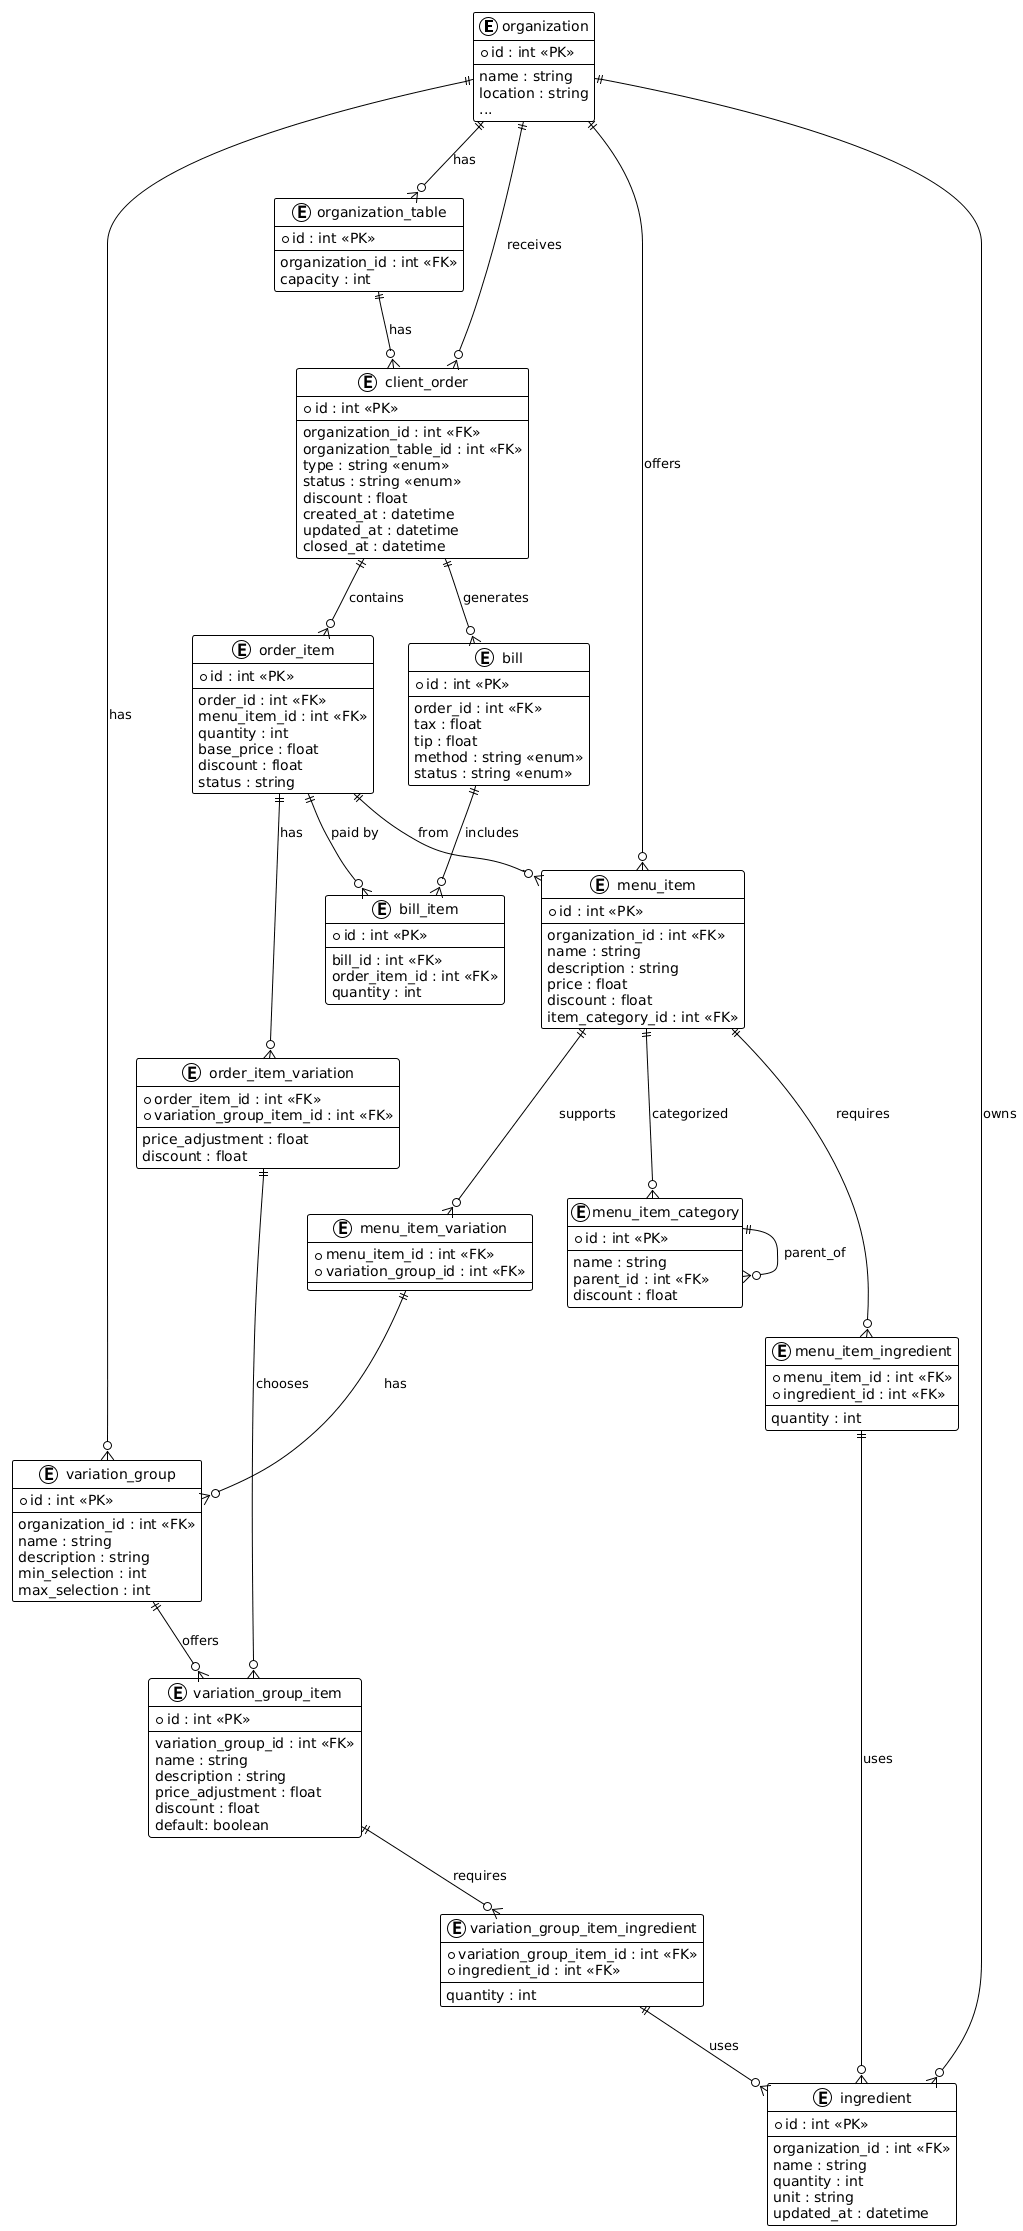
\includegraphics[width=0.65\textwidth]{docs/ps-design/design-document/images/diagrams/orders/order_model_class.png}
    \caption{Order Class Diagram}
    \label{fig:order_class_diagram}
\end{figure}

\subsubsection{Business Data Model}

\paragraph{Design Decisions (Summary)}

Below are the initial data design decisions for business and user account management. 
\begin{itemize}
    \item \textbf{User role-based access control (RBAC):} Roles group permissions, and users are assigned to roles. Also allow per-business role assignment.
    \item \textbf{Identifiers and timestamps:} Use UUID primary keys and maintain \texttt{created} and \texttt{updated\_at} timestamps. This supports managing multiple businesses, potentially distributed across systems.
    \item \textbf{Password security:} Store only hashed passwords. Include fields \texttt{password\_hash}, \texttt{password\_algo/version}, and \texttt{password\_changed\_at}. Do not store plaintext passwords or use reversible encryption.
    \item \textbf{Audit logging:} Track login attempts, password resets, and administrator or manager actions.
    \item \textbf{Support sessions or tokens:} Either server-side session store or JWT approach.
    \item \textbf{Soft-delete:} For users with \textbf{is\_active} and \textbf{deleted\_at} attributes.
\end{itemize}
\textit{RBAC = Role-Based Access Control}

\paragraph{Entities and Tables}  

The database schema is organized into the following entities and supporting tables:  

\begin{itemize}
    \item \textbf{organization}  
    \begin{itemize}
        \item id (PK), name, metadata, created\_at, updated\_at
    \end{itemize}
    \item \textbf{businesses}  
    \begin{itemize}
        \item id (PK), organization\_id (FK), name, metadata, created\_at, updated\_at
    \end{itemize}
    \item \textbf{users}  
    \begin{itemize}
        \item id (PK), organization\_id (FK), business\_id (FK, optional), email, display\_name, username, 
        password\_hash, password\_algo, password\_version, is\_active, email\_verified, last\_login\_at, 
        failed\_login\_attempts, locked\_until, created\_at, updated\_at
    \end{itemize}
    \item \textbf{roles}  
    \begin{itemize}
        \item id (PK), name, description, created\_at
    \end{itemize}
    \item \textbf{permissions}  
    \begin{itemize}
        \item id (PK), name, description
    \end{itemize}
    \item \textbf{role\_permissions}  
    \begin{itemize}
        \item role\_id (FK), permission\_id (FK)
    \end{itemize}
    \item \textbf{user\_roles}  
    \begin{itemize}
        \item user\_id (FK), role\_id (FK), assigned\_by (FK), assigned\_at
    \end{itemize}
    \item \textbf{user\_business\_roles}  
    \begin{itemize}
        \item user\_id (FK), business\_id (FK), role\_id (FK), assigned\_by (FK), assigned\_at
    \end{itemize}
    \item \textbf{sessions}  
    \begin{itemize}
        \item id (PK), user\_id (FK), session\_token, user\_agent, ip, created\_at, last\_seen\_at, expires\_at, revoked
    \end{itemize}
    \item \textbf{password\_resets}  
    \begin{itemize}
        \item id (PK), user\_id (FK), reset\_token, expires\_at, used\_at
    \end{itemize}
    \item \textbf{audit\_logs}  
    \begin{itemize}
        \item id (PK), user\_id (subject, FK), actor\_id (FK), action, resource\_type, resource\_id, details, created\_at
    \end{itemize}
\end{itemize}

\textit{PK = Primary Key,}
\textit{FK = Foreign Key}

\paragraph{Relationships}

Below are the relationships between tables and entities in this schema.
\begin{itemize}
    \item \textbf{Organization $\rightarrow$ Businesses}. One organization can own many businesses. This models a parent company with multiple branches.
    \item \textbf{Organization $\rightarrow$ Users}. One organization can have many users. Users are scoped to an organization.
    \item \textbf{Businesses $\rightarrow$ Users (Optional)}. Users may also have a default \textbf{business\_id} to the business if are tied to one. But users don't have to be tied to a single business. They might be org-level (super admin or a lead manager).
    \item \textbf{Businesses $\rightarrow$ User Store Roles}. A business can have many \textbf{user\_store\_roles}. This lets the assignment of roles to specific businesses.
    \item \textbf{Users $\rightarrow$ Sessions}. One user can have many sessions (logins). Tracks IPs, session tokens, devices.
    \item \textbf{Users $\rightarrow$ User Roles (Organization-wide)}. A user can have many roles at the organization level.
    \item \textbf{Users $\rightarrow$ User Business Roles}. A user can have different roles in different businesses.
    \item \textbf{Users $\rightarrow$ Audit Logs}. A user can generate many audit log entries as an actor. A user can also be the subject of audit logs.
    \item \textbf{Roles $\rightarrow$ Role Permissions}. One role can have many permissions.
    \item \textbf{Permissions $\rightarrow$ Role Permissions}. One permission can belong to many roles.
    \item \textbf{Roles $\rightarrow$ User Roles}. A role can be assigned to many users throughout the organization.
    \item \textbf{Roles $\rightarrow$ User Business Roles}. A role can be assigned to many users within a specific business.
\end{itemize}

\begin{figure}[H]
    \centering
    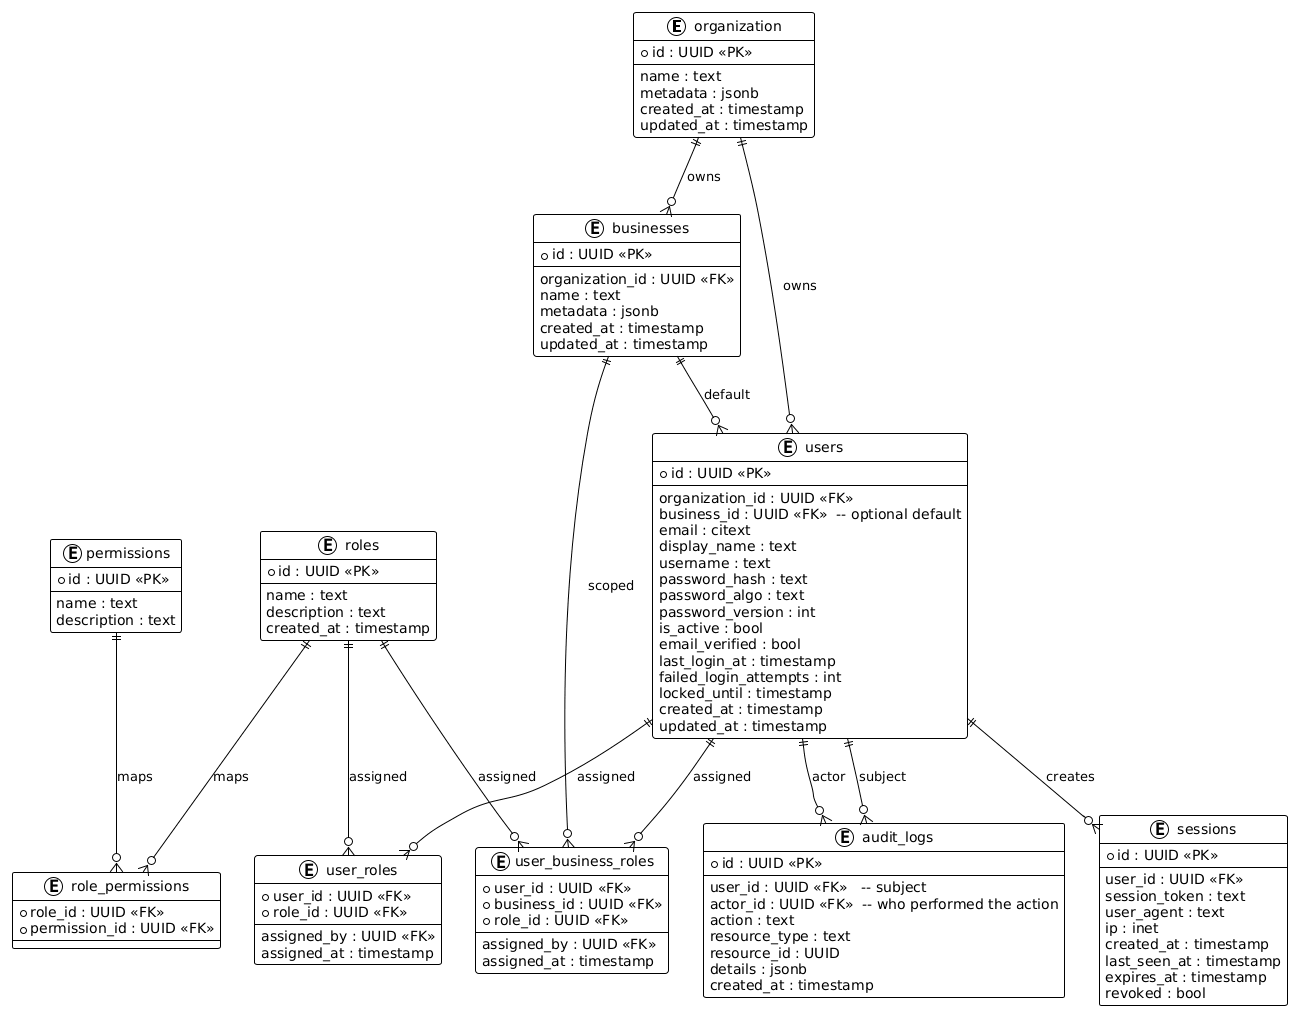
\includegraphics[width=0.8\textwidth]{images/diagrams/business/data_model_business.png}
    \caption{Business Class Diagram with Attributes}
    \label{fig:business_class_diagram}
\end{figure}
This diagram represents different relationships between different entities as well as their attributes. 

\printbibliography[title = {References and sources}]

\end{document}
